% !TEX root = paper.tex

\vspace{4mm}
\epigraph{\textit{``Sometimes you can't see how important something is in its moment, even if it seems kind of important. This is probably one of those times.''}}{(Cyber Grand Challenge highlights from DEF CON 24, August 6, 2016)}

\vspace{-4mm}
\section{Introduction}
\label{se:intro}

%K-ICRS75
Symbolic execution is a popular program analysis technique introduced in the mid '70s to test whether certain properties can be violated by a piece of software~\cite{K-CACM76, SELECT-ICRS75,H-TSE77}. Aspects of interest could be that no division by zero is ever performed, no {\tt NULL} pointer is ever dereferenced, no backdoor exists that can bypass authentication, etc. While in general there is no automated way to decide some properties (e.g., the target of an indirect jump), heuristics and approximate analyses can prove useful in practice in a variety of settings, including mission-critical and security applications.

%While in general there is no automated way to decide some properties (think, e.g., of the halting problem), decidable approximations often exist (e.g., ``does a program always terminate within a certain amount of time?''). Such approximations can prove useful in practice in a variety of settings, including mission-critical and security applications.

In a concrete execution, a program is run on a specific input and a single control flow path is explored. Hence, in most cases concrete executions can only underapproximate the analysis of the property of interest. In contrast, symbolic execution can simultaneously explore multiple paths that a program could take under different inputs. This paves the road to sound analyses that can yield strong guarantees on the checked property. 
The key idea is to allow a program to take on {\em symbolic} -- rather than concrete -- input values. Execution is performed by a {\em symbolic execution engine}, which maintains for each explored control flow path: (i) a first-order Boolean {\em formula} that describes the conditions satisfied by the branches taken along that path, and (ii) a {\em symbolic memory store} that maps variables to symbolic expressions or values. Branch execution updates the formula, while assignments update the symbolic store. A {\em model checker}, typically based on a {\em satisfiability modulo theories} (SMT) solver~\cite{HandbookOfSAT2009}, is used to verify whether there are any violations of the property along each explored path and if the path itself is realizable, i.e., if its formula can be satisfied by some assignment of concrete values to the program's symbolic arguments.

%Variables and control flow paths are associated with expressions and constraints in terms of those symbols during a symbolic execution of the program, and constraints are eventually solved via SMT (satisfiability modulo theories) solvers.

Symbolic execution techniques have been brought to the attention of a heterogenous audience since DARPA announced in 2013 the Cyber Grand Challenge, a two-year competition seeking to create automatic systems for vulnerability detection, exploitation, and patching in near real-time~\cite{ANGR-SSP16}.
More remarkably, symbolic execution tools have been running 24/7 in the testing process of many Microsoft applications since 2008, revealing, e.g., nearly 30\% of the bugs discovered during the development of Windows 7, which other analyses and blackbox testing techniques missed~\cite{SAGE-QUEUE12}.

%In this article, we survey the main aspects of symbolic execution and discuss its extensive usage in software testing and computer security applications, where software vulnerabilities can be found by symbolically executing programs at the level of either source or binary code. We start with a simple example that highlights many of the fundamental issues addressed in the remainder of the article.

In this paper, we describe the main aspects of symbolic execution and the scalability problems it typically encounters. We discuss its extensive usage in software testing and computer security applications, where software is often available in binary form only. We start with a simple example that highlights many of the fundamental issues that arise when executing code symbolically.

% --------------------------------------------------------------------------------------------------------------------
\section{A Warm-up Example}
\label{symbolic-execution-example}

Consider the C code of Figure~\ref{fig:example-1} and assume that our goal is to determine which inputs make the  {\tt assert} at line 8 of function \texttt{foobar} fail. Since each input parameter can take as many as $2^{32}$ distinct integer values, the approach of running concretely function \texttt{foobar} on randomly generated inputs will unlikely pick up exactly the assert-failing inputs.
%Techniques such as random testing could generate bottomless input tests for this function. 
%However, it is unlikely that exactly the assert-failing inputs would be randomly picked up\mynote{Fuzzing?}. 
By evaluating the code using symbols for its inputs, instead of concrete values, symbolic execution overcomes this limitation and makes it possible to reason on {\em classes of inputs}, rather than single input values. 

\begin{figure}[t]
\begin{center}
\begin{tabular}{c}
\begin{lstlisting}[basicstyle=\ttfamily\scriptsize]
1.  void foobar(int a, int b) {
2.     int x = 1, y = 0;
3.     if (a != 0) {
4.        y = 3+x;
5.        if (b == 0)
6.           x = 2*(a+b);
7.     }
8.     assert(x-y != 0);
9.  }
\end{lstlisting}
\end{tabular}
\end{center}
\vspace{-2mm}
\caption{Warm-up example: which values of \texttt{a} and \texttt{b} make the \texttt{assert} fail?}
\label{fig:example-1}
\end{figure}

In more detail, every value that cannot be determined by a static analysis of the code, such as an actual parameter of a function or the result of a system call that reads data from a stream, is represented by a symbol $\alpha_i$. At any time, the symbolic execution engine maintains a state $(stmt,~\sigma,~\pi)$ where:

\begin{itemize}

%\item $stmt$ is the next statement to evaluate. For the time being, we assume that $stmt$ can be an assignment, a conditional branch, or a jump (more complex constructs such as function calls and loops will be discussed in  Section~\ref{se:executors} and Section~\ref{se:loops}, respectively).
\item $stmt$ is the next statement to evaluate. For the sake of simplicity, we assume that $stmt$ can be an assignment, a conditional branch, or a jump.

\item $\sigma$ is a {\em symbolic store} that associates program variables with either expressions over concrete values or symbolic values $\alpha_i$.

\item $\pi$ denotes the {\em path constraints}, i.e., is a formula that expresses a set of assumptions on the symbols $\alpha_i$ due to branches taken in the execution to reach $stmt$. At the beginning of the analysis, $\pi=true$.

\end{itemize}

\noindent Depending on $stmt$, the symbolic engine changes the state as follows:

\begin{itemize}[topsep=4pt] % TODO
  \item The evaluation of an assignment $x=e$ updates the symbolic store $\sigma$ by associating $x$ with a new symbolic expression $e_s$. We denote this association with $x\mapsto e_s$, where $e_s$ is obtained by evaluating $e$ in the context of the current execution state and  can be any expression involving unary or binary operators over symbols and concrete values.
  
%   $\alpha_i = e$: when an expression $e$ is assigned to a symbol $\alpha_i$, $pc$ is extended by adding a constraint on $\alpha_i$:
%    \[ pc \gets pc \wedge \alpha_i = e\]
%  where $e$ can be any expression, involving unary or binary operators, over symbols and constants.

  \item The evaluation of a conditional branch ${\tt if}~e~{\tt then}~s_{true}~{\tt else}~s_{false}$ affects the path constraints $\pi$. The symbolic execution is forked by creating two execution states with path constraints $\pi_{true}$ and $\pi_{false}$, respectively, which correspond to the two branches: $\pi_{true}=\pi \wedge e_s$ and $\pi_{false}=\pi \wedge \neg e_s$, where $e_s$ is a symbolic expression obtained by evaluating $e$. 
%        \[ (s_{true}, pc_{true}) \text{ where } pc_{true} = pc \wedge e \]
%        \[ (s_{false}, pc_{false}) \text{ where } pc_{false} = pc \wedge \neg e \]
    Symbolic execution proceeds independently on both states.

  \item The evaluation of a jump {\tt goto} $s$ updates the execution state by advancing the symbolic execution to statement $s$. 
\end{itemize}

\begin{figure}[t]
  \centering
  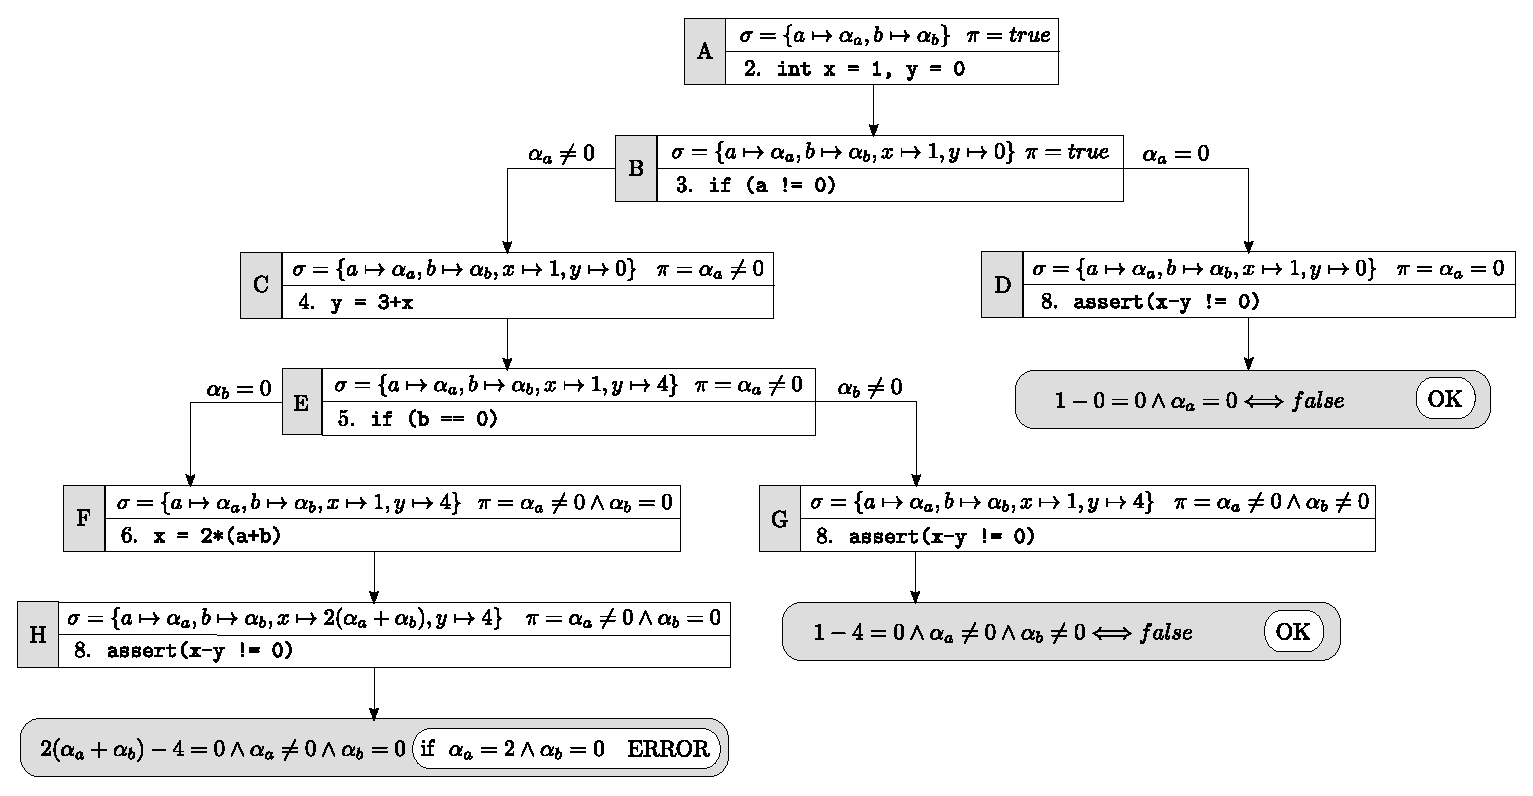
\includegraphics[width=1.0\columnwidth]{images/execution-tree.eps} 
  \caption{Symbolic execution tree of function {\tt foobar} given in Figure~\ref{fig:example-1}. Each execution state, labeled with an upper case letter, shows the statement to be executed, the symbolic store $\sigma$, and the path constraints $\pi$. Leaves are evaluated against the condition in the {\tt assert} statement. }
%For the sake of presentation the conjunction of constraints is shown as a list of constraints. }
  \label{fig:example-symbolic-execution}
\end{figure}

\noindent A symbolic execution of function {\tt foobar}, which can be effectively represented as a tree, is shown in Figure~\ref{fig:example-symbolic-execution}. Initially (execution state $A$) the path constraints are {\tt true} and input arguments {\tt a} and {\tt b} are associated with symbolic values. 
After initializing local variables {\tt x} and {\tt y} at line 2, the symbolic store is updated by associating {\tt x} and {\tt y} with concrete values 1 and 0, respectively (execution state $B$). Line 3 contains a conditional branch and the execution is forked: depending on the branch taken, a different statement is evaluated next and different assumptions are made on symbol $\alpha_a$ (execution states $C$ and $D$, respectively). In the branch where $\alpha_a\neq 0$, variable {\tt y} is assigned with ${\tt x}+3$, obtaining $y\mapsto 4$ in state $E$ because $x\mapsto 1$ in state $C$. In general, arithmetic expression evaluation simply manipulates the symbolic values.
After expanding every execution state until the {\tt assert} at line 8 is reached on all branches, we can check which input values for parameters {\tt a} and {\tt b} can make the {\tt assert} fail. By analyzing execution states $\{D,G,H\}$, we can conclude that only $H$ can make {\tt x-y = 0} true. The path constraints for $H$ at this point implicitly define the set of inputs that are unsafe for {\tt foobar}. 
In particular, any input values such that:
 \[ 2(\alpha_a+\alpha_b)-4 = 0 \wedge \alpha_a \neq 0 \wedge \alpha_b = 0 \]
will make {\tt assert} fail. An instance of unsafe input parameters can be eventually determined by invoking a {\em model checker}~\cite{HandbookOfSAT2009} to solve the path constraints, which in this example would yield $a = 2$ and $b = 0$. 

%Notice\mynote{Say earlier?} that a constraint solver is also needed when evaluating the satisfiability of branch conditions.

% --------------------------------------------------------------------------------------------------------------------
\section{Challenges in Symbolic Execution}
\label{example-discussion}

In the example discussed in Section~\ref{symbolic-execution-example} symbolic execution can identify {\em all} the possible unsafe inputs that make the {\tt assert} fail. This is achieved through an exhaustive exploration of the possible execution states. From a theoretical perspective, exhaustive symbolic execution provides a {\em sound} and {\em complete} methodology for any decidable analysis. Soundness prevents false negatives, i.e., all possible unsafe inputs are guaranteed to be found, while completeness prevents false positives, i.e.,  input values deemed as unsafe are actually unsafe. As we will discuss later on, exhaustive symbolic execution is unlikely to scale beyond small applications. Hence, in practice we often settle for less ambitious goals, e.g., by trading soundness for performance.

Challenges that symbolic execution has to face when processing real-world code can be significantly more complex than those illustrated in our warm-up example. In the remainder of this section, we address a number of observations and questions that naturally arise.

% !TEX root = main.tex


%%%%%%%%%%%%%%%%%%%%%%%%%%%%%%%%%%%%%%%%%%%%%%%%%%%%%%%%%%%
\section{Memory model}
\label{memory-model}

Our warm-up example of Section~\ref{symbolic-execution-example} presented a simplified memory model where data are stored in scalar variables only, with no indirection. A crucial aspect of symbolic execution is how memory should be modeled to support programs with pointers and arrays. This requires extending our notion of memory store by mapping not only variables, but also memory addresses to symbolic expressions or concrete values. In general, a store $\sigma$ that explicitly models memory addresses can be thought as a mapping that associates memory addresses (indexes) with either expressions over concrete values or symbolic values. We can still support variables by using their address rather than their name in the mapping. In the following, when we write $x\mapsto e$ for a variable $x$ and an expression $e$ we mean $\&x\mapsto e$, where $\&x$ is the concrete address of variable $x$. Also, if $v$ is an array and $c$ is an integer constant, by $v[c]\mapsto e$ we mean $\&v+c\mapsto e$. A memory model is an important design choice for a symbolic engine, as it can have a significant influence on the coverage achieved by symbolic execution, as well as on the scalability of constraint solving~\cite{CS-CACM13}.

The {\em symbolic memory address} problem~\cite{SAB-SP10} arises when the address referenced in the operation is a symbolic expression. In the remainder of this section, we discuss a number of popular solutions.

\subsection{Fully Symbolic Memory}
\label{ss:fully-symbolic-memory}

At the one end of the spectrum, an engine may treat memory addresses as fully symbolic. This is the approach taken by a number of works (e.g., {\sc BitBlaze}~\cite{BITBLAZE-ICISS08},~\cite{TLL-CAV10}, {\sc BAP}~\cite{BAP-CAV11}, and~\cite{TS-ATVA14}). Two fundamental approaches, pioneered by King in its seminal paper~\cite{K-CACM76}, are the following:

\begin{itemize}

\item {\em State forking.} If an operation reads from or writes to a symbolic address, the state is forked by considering all possible states that may result from the operation. The path constraints are updated accordingly for each forked state.
\boxedexample{Consider the example shown in Figure~\ref{fi:example-mem}. The write operation at line 4 affects either $a[0]$ or $a[1]$, depending on the unknown value of array index $i$. State forking creates two states after executing the memory assignment to explicitly consider both possible scenarios (Figure~\ref{fi:memory-fork}). The path constraints for the forked states encode the assumption made on the value of $i$. Similarly, the memory read operation \texttt{a[j]} at line 5 may access either $a[0]$ or $a[1]$, depending on the unknown value of array index $j$. Therefore, for each of the two possible outcomes of the assignment \texttt{a[i]=5}, there are two possible outcomes of the \texttt{assert}, which are explicitly explored by forking the corresponding states. }

\begin{figure}[ht]
\begin{center}
\begin{tabular}{c}
\begin{lstlisting}[basicstyle=\ttfamily\scriptsize]
1.  void foobar(unsigned i, unsigned j) {
2.     int a[2] = { 0 };
3.     if (i>1 || j>1) return;
4.     a[i] = 5;
5.     assert(a[j] != 5);
6.  }
\end{lstlisting}
\end{tabular}
\end{center}
\vspace{-2mm}
\caption{Memory modeling example: which values of \texttt{i} and \texttt{j} make the \texttt{assert} fail?}
\label{fi:example-mem}
\end{figure}

\begin{figure}[ht]
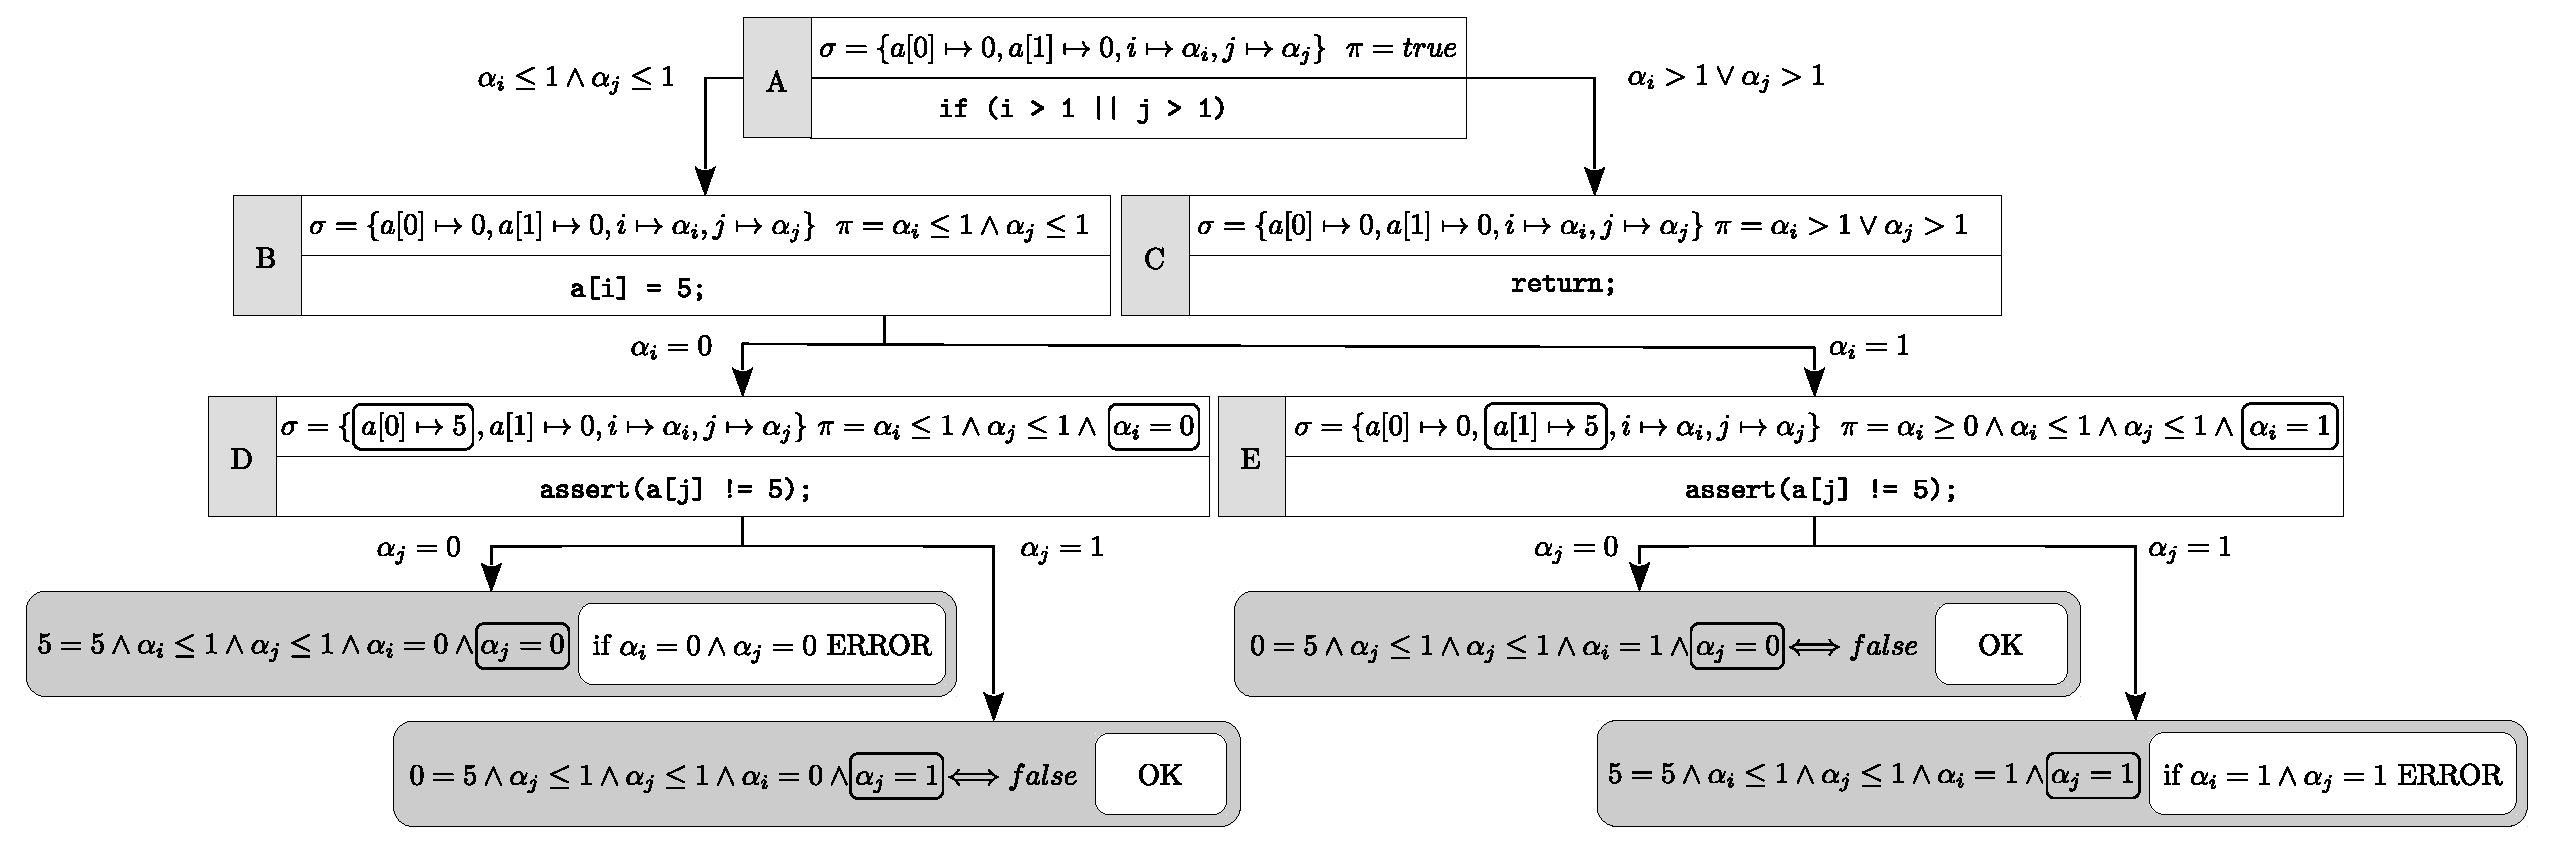
\includegraphics[width=1\columnwidth]{images/memory-fork} 
\vspace{-4.5mm}
\caption{Fully symbolic memory via state forking for the example of Figure~\ref{fi:example-mem}.}
\label{fi:memory-fork}
\end{figure}

\item {\em if-then-else formulas.} An alternative approach consists in encoding the uncertainty on the possible values of a symbolic pointer into the expressions kept in the symbolic store and in the path constraints, without forking any new states. The key idea is to exploit the capability of some solvers to reason on formulas that contain if-then-else expressions of the form $ite(\texttt{c}, \texttt{t}, \texttt{f})$, which yields \texttt{t} if \texttt{c} is true, and \texttt{f} otherwise\footnote{In propositional logic, the $ite(\texttt{c}, \texttt{t}, \texttt{f})$ expression could be replaced with the formula $(\texttt{c} \wedge \texttt{t}) \vee (\neg\texttt{c} \wedge \texttt{f})$.}.
The approach works differently for memory read and write operations. Let $\alpha$ be a symbolic address that may assume the concrete values $a_1, a_2, \ldots$:
\begin{itemize}
\item reading from $\alpha$ yields the expression $ite(\alpha=a_1,\sigma(a_1), ite(\alpha=a_2,\sigma(a_2), \ldots))$;
\item writing an expression $e$ at $\alpha$ updates the symbolic store for each $a_1, a_2, \ldots$ as $\sigma(a_i)\gets ite(\alpha=a_i,e,\sigma(a_i))$.
\end{itemize}
Notice that in both cases, a memory operation introduces in the store as many $ite$ expressions as the number of possible values the accessed symbolic address may assume. The $ite$ approach to symbolic memory is used, e.g., in {\sc Angr}~\cite{ANGR-SSP16} (Section~\ref{ss:index-based-memory}).
\boxedexample{Consider again the example shown in Figure~\ref{fi:example-mem}. Rather than forking the state after the operation \texttt{a[i]=5} at line 4, the if-then-else approach updates the memory store by encoding both possible outcomes of the assignment, i.e., $a[0]\mapsto ite(\alpha_i=0,5,0)$ and $a[1]\mapsto ite(\alpha_i=1,5,0)$ (Figure~\ref{fi:memory-ite}). Similarly, rather than creating a new state for each possible distinct address of \texttt{a[j]} at line 5, the uncertainty on $j$ is encoded in the single expression $ite(\alpha_j=0,\sigma(a[0]),\sigma(a[1]))=ite(\alpha_j=0,ite(\alpha_i=0,5,0),ite(\alpha_i=1,5,0))$.
%: if $\alpha_i=0$ then $a[0]\mapsto 5$ and $a[1]\mapsto 0$; conversely, if $\alpha_i=1$ then $a[0]\mapsto 0$ and $a[1]\mapsto 5$.
%State forking creates two states after executing the memory assigment to explicitly consider both possible scenarios (Figure~\ref{fi:memory-fork}). The path constraints for the forked states encode the assumption made on the value of $i$. Similarly, the memory read operation \texttt{a[j]} at line 5 may access either $a[0]$ or $a[1]$, depending on the unknown value of array index $j$. Therefore, for each of the two possible outcomes of the assignment \texttt{a[i]=5}, there are two possible outcomes of the \texttt{assert}, which are explicitly explored by forking the corresponding states. 
}

%Indeed, the $ite(\texttt{c}, \texttt{t}, \texttt{f})$ expression introduced in the symbolic store $\sigma$ is a short term for an {\tt if-then-else} expression and means that if the condition {\tt c} is verified then {\tt t} holds, otherwise {\tt f} must be assumed as true. Nonetheless, $ite$ expressions are often just syntactic sugar for disjunctive formulas and are commonly supported by most prominent constraint solvers. For instance, in the context of propositional logic the $ite(\texttt{c}, \texttt{t}, \texttt{f})$  expression could be replaced with the formula $(\texttt{c} \wedge \texttt{t}) \vee (\neg\texttt{c} \wedge \texttt{f})$ . 

\end{itemize}

\begin{figure}[t]
\begin{center}
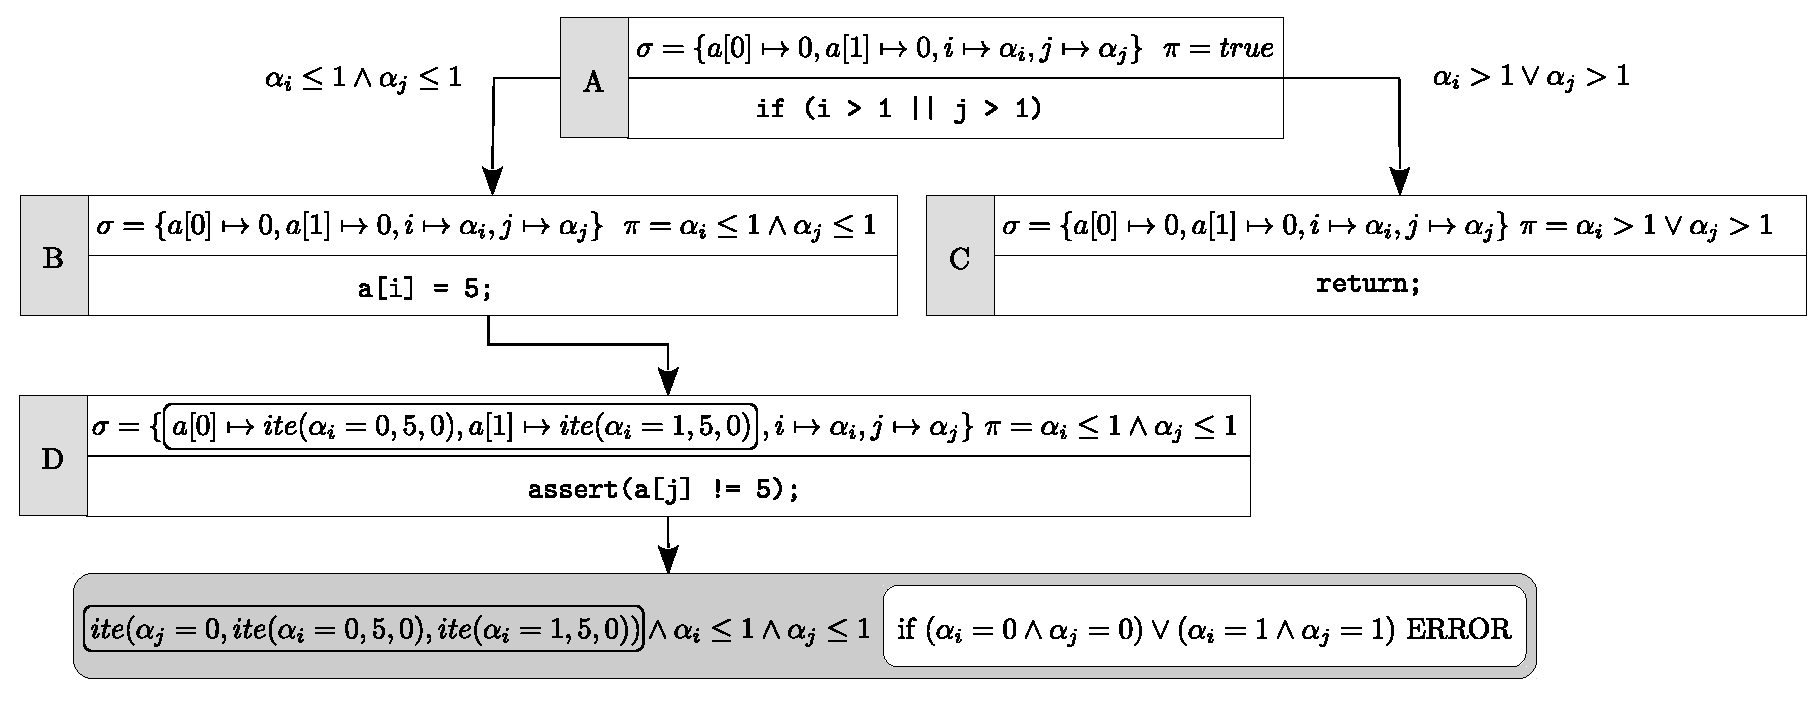
\includegraphics[width=0.7\columnwidth]{images/memory-ite} % TODO 0.7
\end{center}
\vspace{-2.5mm}
\caption{Fully symbolic memory via if-then-else formulas for the example of Figure~\ref{fi:example-mem}.}
%\vspace{-1mm} % TODO
\label{fi:memory-ite}
\end{figure}

\noindent In general, a symbolic address may reference any cell in memory, making the approaches described above intractable. Fortunately, in many practical cases the set of possible addresses a memory operation may reference is small~\cite{BITBLAZE-ICISS08}, as in the example shown in Figure~\ref{fi:example-mem} where indexes $i$ and $j$ range in a bounded interval. 

%Reasoning about all possible values a pointer may assume is notoriously hard, as in the worst case a symbolic address may reference any cell in memory. In most cases, however, symbolic memory accesses are typically already constrained to small ranges~\cite{BITBLAZE-ICISS08}. \mynote{Cite VSA \& aliasing as refinements? -- VSA is discussed below} Hence, an engine can ask the solver for the range of possible values for an address in order to restrict the exploration. 

%When obtained ranges are too large, {\sc BitBlaze}~\cite{BITBLAZE-ICISS08} adds a further constraint to the system to limit its size. However, the authors observe that most symbolic memory accesses are typically already constrained to small ranges in practice, making it unnecessary.

To model fully symbolic pointers, an extensive line of research  (e.g., {\sc EXE}~\cite{EXE-CCS06}, {\sc KLEE}~\cite{KLEE-OSDI08}, {\sc SAGE}~\cite{EGL-ISSTA09}) leverages the expressive power of some SMT solvers, which can model operations on arrays as first-class entities in constraint formulas using {\em theories of arrays} in their decision procedures~\cite{STP-CAV07}. 

%\vspace{-2pt} % TODO
\subsection{Address Concretization}
\label{ss:address-concretization}

In all cases where the combinatorial complexity of the analysis explodes as pointer values cannot be bounded to sufficiently small ranges, {\em address concretization}, which consists in concretizing a pointer to a single specific address, is a popular alternative. This can reduce the number of states and the complexity of the formulas fed to the solver and thus improve running time, although may cause the engine to miss paths that, for instance, depend on specific values for some pointers. 

%\mynote{DART is mentioned in CS-CACM13 as  using theories of arrays} --> added to the list above.
Concretization arises naturally in offline executors (Section~\ref{ss:principles}). Prominent examples are {\sc DART}~\cite{DART-PLDI05} and early {\sc SAGE} releases~\cite{SAGE-NDSS08} that concretely execute one path at a time while collecting path constraints along executed paths. %\mynote{[D] was: equality and inequality}  
Systems such as {\sc CUTE}~\cite{CUTE-FSE13} and {\sc CREST}~\cite{CREST-ASE08} are capable of reasoning only about equality constraints for pointers, as they can be solved efficiently, and resort to concretization for general symbolic references. % equality and inequality

%we normally get or set a concrete value at a particular memory address. When executing symbolically, a design choice for a symbolic engine concerns what to do when a memory reference is an expression instead of a concrete address.

%\subsection{Theory of Arrays}
%\label{ss:theory-arrays}

%A number of works (e.g., {\sc EXE}~\cite{EXE-CCS06}, {\sc KLEE}~\cite{KLEE-OSDI08}, and {\sc SAGE}~\cite{SAGE-NDSS08}) model pointers using the theory of arrays available from SMT decision procedures. 

%In this section we provide a description of its implementation in the popular STP solver~\cite{STP-CAV07}.

%The design of STP has been mainly driven by the demands of research projects on software analysis. Its input language supports one-dimensional arrays that are indexed by bitvectors and contain bitvectors. Given an array $A$, a $read(A,i)$ operation returns the value $A[i]$ at the location expressed by the index $i$, while a $write(A,i,v)$ returns a new array with the same values as $A$ at all indexes except $i$, where it contains the value $v$. Array reads and write typically appear as subexpressions of an $ite(c,a,b)$ expression, which is syntactic sugar for $(if\,c\;then\,b\;else\,a)$.

%STP reduces formulas over array to an equisatisfiable form that contains no $read$ or $write$ operations by applying three standard transformations and introducing fresh bitvector variables. Generated formulas are then amenable to SAT solving. However, transformations can also introduce bottlenecks, for instance by destroying sharing of subterms, and thus are typically procrastinated using refinement algorithms. SMT attempts also to eliminate variables through linear solving~\cite{STP-CAV07}.

%\vspace{-2pt} % TODO
\subsection{Partial Memory Modeling}
\label{ss:index-based-memory}

To mitigate the scalability problems of fully symbolic memory and the loss of soundness of memory concretization,
%Motivated by the observation that concretizing all memory indexes might not work well in some scenarios, while fully symbolic memory does not scale, 
{\sc Mayhem}~\cite{MAYHEM-SP12} explores a middle point in the spectrum by introducing a {\em partial} memory model. The key idea is that written addresses are always concretized and read addresses are modeled symbolically if the contiguous interval of possible values they may assume is small enough. This model is based on a trade-off: it uses more expressive formulas than concretization, since it encodes multiple pointer values per state, but does not attempt to encode all of them like in fully symbolic memory~\cite{MAYHEM-THESIS}. A basic approach to bound the set of possible values that an address may assume consists in trying different concrete values and checking whether they satisfy the current path constraints, excluding large portions of the address space at each trial until a tight range is found.  
%This choice is important to keep the analysis feasible: for instance, in a fully symbolic model a repeated read and write on the same symbolic index would result in quadratic increase in either the symbolic constraints or the complexity of the stored symbolic expressions~\cite{DRILLER-NDSS16}.
%Global memory is defined as a map $\mu$ from 32-bit addresses ({\em indexes}) to expressions. When a symbolic index $i$ is used to read memory, the algorithm generates a memory object $M$ containing the projection of $\mu$ over all the valid values that $i$ can assume. The evaluation of a $load(\mu,i)$ operation is thus reduced to $M[i]$, where $M$ is typically orders of magnitude smaller than the entire memory $\mu$.
%Instantiating a memory object still requires finding all the possible values for a symbolic index. A naive algorithm would employ the constraint solver to refine the range of an index using binary search under the current path constraints. 
This algorithm comes with a number of caveats: for instance, querying the solver on each symbolic dereference is expensive, the memory range may not be continuous, and the values within the memory region of a symbolic pointer might have structure. {\sc Mayhem}~\cite{MAYHEM-SP12} thus performs a number of optimizations, including Value Set Analysis~\cite{VSA-CC04} and forms of query caching (Section~\ref{se:constraint-solving}), to refine ranges efficiently. If at the end of the process the range size exceeds a given threshold (e.g., 1024), the address is concretized. {\sc Angr}~\cite{ANGR-SSP16} also adopts the partial memory model idea and extends it by optionally supporting write operations on symbolic pointers that range within small contiguous intervals (up to 128 addresses). % [D] ptr may also be redirected to symbolic data

%%%%%%%%%%%%%%%%%%%%%%%%%%%%%%%%%%%%%%%%%%%%%%%%%%%%
\subsection{Complex Objects}
\label{ss:complex-objects}

\mytempedit{\myparagraph{Lazy Initialization}}
\cite{KPV-TACAS03} propose symbolic execution techniques for advanced object-oriented language constructs, such as those offered by C++ and Java. The authors describe a framework for software verification that combines symbolic execution and model checking to handle linked data structures such as lists and trees. % [D] added dynamically allocated & discarded primitive data types, and concurrency.

In particular, they generalize symbolic execution by introducing {\em lazy initialization} to effectively handle dynamically allocated objects. Compared to our warm-up example (Section~\ref{symbolic-execution-example}), the state representation is extended with a {\em heap configuration} used to maintain such objects. Symbolic execution of a method taking complex objects as inputs starts with uninitialized fields, and assigns values to them in a lazy fashion, i.e., they are initialized when first accessed during execution.

When an uninitialized reference field is accessed, the algorithm forks the current state with three different heap configurations, in which the field is initialized with: (1) {\tt null}, (2) a reference to a new object with all symbolic attributes, and (3) a previously introduced concrete object of the desired type, respectively. This on-demand concretization enables symbolic execution of methods without the need for any previous knowledge on the number of objects given as input. Also, forking the state as in (2) results into a systematic treatment for aliasing, i.e., when an object can be accessed through multiple references.

\cite{KPV-TACAS03,SPF-ISSTA04} combine lazy initialization with user-provided {\em method preconditions}, i.e., conditions which are assumed to be true before the execution of a method. Preconditions are used to characterize those program input states in which the method is expected to behave as intended by the programmer. For instance, we expect a binary tree data structure to be acyclic and with every node - except for the root - having exactly one parent. Conservative preconditions are used to ensure that incorrect heap configurations are eliminated during initialization, speeding up the symbolic execution process.

Further refinements to lazy initialization are described in a number of works, e.g.,~\cite{DLR-ASE12,BLI-NFM13,BLISS-TSE15}, which all share the goal of reducing the number of heap configurations to generate when forking the state.~\cite{DLR-ASE12} also provides a formal treatment of lazy initialization in Java.

\mytempedit{\myparagraph{Verifying Client Code Only}}
Of a different flavor is the technique presented in~\cite{SHZ-TAIC07} for symbolic execution over objects instantiated from commonly used libraries. The authors argue that performing symbolic execution at the representation level might be redundant if the aim is to only check the client code, thus trusting the correctness of the library implementation. They discuss the idea of symbolically executing methods of the Java {\tt String} class using a finite-state automaton that abstracts away the implementation details. They present a case study of an application that dynamically generates SQL queries: symbolic execution is used to check whether the statements conform to the SQL grammar and possibly match injection patterns. \iffullver{The authors mention that their approach might be used to symbolically execute over standard container classes such as trees or maps. It is worth mentioning that symbolic execution is used to detect SQL injection vulnerabilities also in~\cite{FLP-COMPSAC07}.}{The authors mention that their approach might be used to symbolically execute over standard container classes such as trees or maps.}

\mytempedit{
\myparagraph{Separation Logic}
Checking memory safety properties for pointer programs is a major challenge in program verification. Recent years have witnessed {\em separation logic} (SL)~\cite{Reynolds02,IO-POPL01} emerging as one leading approach to reason about heap manipulations in imperative programs. SL extends Hoare logic to support local reasoning for programs that manipulate pointer data structures, and allows for expressing complex invariants of heap configurations in a succinct manner.

% pure (i.e., heap-independent)
SL relies on a {\em separating conjunction} binary operator $*$, which asserts that the heap can be partitioned into two components where its two arguments hold, respectively. For instance, predicate $A * x\mapsto�[n:y]$ says that the heap can be divided into a single cell $x$ that points to a record holding $y$ in its $n$ field, and the rest of the heap where $A$ holds. Program state can be modeled as a {\em symbolic heap} $\Pi\,\brokenvert\,\Sigma$, where $\Pi$ is a finite set of pure predicates accounting for variables while $\Sigma$ is a finite set of heap predicates. Symbolic heaps are treated as SL formulas symbolically executed using an abstract semantics for each statement in the program. A number of rules are typically employed to support entailment of symbolic heaps, to infer which portions of the heap are left unchanged by a statement, and to ensure termination of symbolic execution through by using abstraction (e.g., through a widening operator).

One of the main reasons behind the success of SL lies in the local form of reasoning enabled by its separating conjunction, which allows for specifications that speak only about the memory actually accessed by the code. This also fits together with the goal of deriving inductive definitions aiming at describing mutable data structures. When compared to other verification approaches, the annotation burden on the user is rather little or often absent. For instance, ~\cite{CDO-JACM11} presents a shape analysis based on a generalized form of abduction to automatically discover invariants on data structures and compute composable procedure summaries in SL.

Several tools based on SL are available to date for automatically finding memory bugs in user~\cite{INFER} and system-level code~\cite{SLAYER-CAV11}, and for verifying annotated programs with respect to, e.g., memory safety properties~\cite{VERIFAST-APLAS10} and design patterns~\cite{JSTAR-OOPSLA08}. While tailor-made theorem provers are implemented in many extant tools, recent works~\cite{BPS-ENTCS09,PWZ-CAV13} have shown that provers for decidable fragments of SL can be integrated in an SMT solver, allowing for complete combinations with other theories that are relevant in program verification (Section~\ref{se:constraint-solving}). This paves the way for interesting applications of SL in general-purpose verification tools. In particular, symbolic executors could use it to reason inductively over manipulations of data structures such as lists and trees in C and Java programs. To the best of our knowledge, while symbolic execution is at the core of SL, there have not been applications of SL in symbolic executors yet. We believe this might represent a promising research direction to follow.}

% Additional optimizations are presented in~\cite{DLR-ASE12}, which also provides a complete formalization of this approach for the Java language.

% [D] this is related to input test generation
%Also, generated heap configurations are pairwise non-isomorphic: eliminating symmetric structures can greatly reduce the number of heaps that a symbolic executor must explore, while guaranteeing that no relevant states are missed~\cite{BLISS-TSE15}. 

%~\cite{KPV-TACAS03,SPF-ISSTA04} combine lazy initialization with user-provided {\em method preconditions}, i.e., conditions which are assumed to be true before the execution of a method. Such conditions are used to characterize those input states in which the method is expected to behave as intended by the programmer. For instance, we expect a binary tree data structure to be acyclic and with every node - except for the root - having exactly one parent. Conservative method preconditions are used to ensure that incorrect structures are eliminated during initialization, speeding the symbolic execution process up.

%Further refinements to lazy initialization are described in a number of works. \cite{BLI-NFM13} introduces {\em bounded lazy initialization} (BLI) to reduce the number of alternatives to explore using available field bounds expressed in TACO, a tool for SAT-based bounded verification of JML-annotated Java code. ~\cite{BLISS-TSE15} presents two novel techniques that build upon BLI. The first technique refines field bounds by leveraging information from already-concretized fields; the technique is then extended by  auxiliary satisfiability checks to determine the feasibility of partially symbolic structure.

% !TEX root = paper.tex
%\vspace{-2mm} % TODO
\subsection{Interaction with the Environment}
\label{ss:environment}

Real-world applications constantly interact with the environment (e.g., the file system or the network) through libraries and system calls. These interactions may cause side-effects (e.g., file creation)
that could later affect the execution and must be therefore taken into account. Evaluating any possible interaction outcome is generally unfeasible: it could generate a large number of execution states, of which only a small number can actually happen in a non-symbolic scenario.

%A typical strategy is to consider popular library and system routines and create models that can help the symbolic engine analyze only significant outcomes.

A body of early works (e.g., {\sc DART}~\cite{DART-PLDI05},  {\sc CUTE}~\cite{CUTE-FSE13}, and {\sc EXE}~\cite{EXE-CCS06}) includes the environment in symbolic analysis by actually executing external calls using concrete arguments for them. This indeed limits the behaviors they can explore compared to a fully symbolic strategy, which on the other hand might be unfeasible.
%In an online executor this choice also results in having calls from distinct paths of execution interfere with each other.
This choice might also result in having calls from distinct paths of execution interfere with each other. 

Another way to tackle the problem is to create an abstract model that captures these interactions. For instance, in {\sc KLEE}~\cite{KLEE-OSDI08} symbolic files are supported through a basic {\em symbolic file system} for each execution state, consisting of a directory with $n$ symbolic files whose number and sizes are specified by the user. An operation on a symbolic file results in forking $n+1$ state branches: one for each possible file, plus an optional one to capture unexpected errors in the operation.
%As the number of functions in a standard library is typically large and writing models for them is expensive and error-prone~\cite{Ball06}, models are generally implemented at system call-level rather than library level. This enables the symbolic exploration of the libraries as well.

{\sc AEG}~\cite{AEG-NDSS11} models most of the system environment that could be used by an attacker as input source, including the file system, network sockets, and environment variables. Additionally, more than 70 library and system calls are emulated, including thread- and process-related system calls, and common formatting functions to capture potential buffer overflows. %Symbolic files are handled as in {\sc KLEE}~\cite{KLEE-OSDI08}, while symbolic sockets are dealt with in a similar manner, with packets and their payloads being processed as in symbolic files and their contents. {\sc Cloud9} further extends support to many other POSIX libraries, allowing users to also control advanced conditions in the testing environment. For instance, it can simulate reordering, delays, and packet dropping caused by a fragmented data stream over a network.

%{\sc \stwoe}~\cite{CKC-TOCS12} remarks that models, other than expensive to write, rarely achieve full accuracy, and may quickly become stale if the modeled system changes.
{\sc \stwoe}~\cite{CKC-TOCS12} remarks that models are expensive to write and rarely achieve full accuracy.
In their platform, the authors rely on virtualization to perform the desired analysis on the real software stack, preventing side effects from propagating across independent execution paths. 

% !TEX root = main.tex

\section{Loops}
\label{se:loops}

Loops are one of the main cause of path explosion: each iteration of a loop can be seen as a {\tt IF-GOTO} statement, leading to a conditional branch in the execution tree. If the loop condition involves one or more symbolic values, the number of generated branches may be potentially infinite. For instance, consider the following example (taken from~\cite{CS-CACM13}):
    \begin{lstlisting}[basicstyle=\ttfamily\small]
    1.  int N = sym_input(); // e.g., read from file
    2.  while (N > 0) {
    3.    N = sym_input();  
    4.  }
    \end{lstlisting}
where \texttt{sym\_input()} ... The path constraint set of any final state will contain:
  \[ \left ( \bigwedge_{i \in [1, k]]} N_i > 0 \right ) \wedge (N_{k+1} \leq 0) \]
where  $k$ is the number of iterations and $N_i$ is the symbol introduced at the $i$-th iteration.\\

The problem of path explosion due to symbolic execution of loops has been attacked from different sides. A first natural strategy adopted by many symbolic engines is to limit the loop exploration up to a certain number of iterations. Obviously, this may lead to missing interesting paths in the program. For this reason, some works (e.g., ~\cite{AEG-NDSS11}) have also considered the opposite strategy, allowing the engine to fully explore some loops. Indeed, this has been shown to be effective in some application contexts such as security (e.g., identification of buffer overflows) where interesting behaviour may be observed at the loop boundaries.

By using static or dynamic analysis techniques, it may be possible to derive properties over a loop that can be exploited by the symbolic engine to significantly prune branching paths. For instance, knowledge of the exact number of loop iterations - or at least a constant upper bound on it - can significantly help the engine. Section~\ref{precontioned-symbolic-execution} provides a more general discussion of how preconditions can help symbolic execution.

% prior works; assertion (i.e., a property that should hold)
Some works have instead proposed to replace in the symbolic execution tree the possibly infinite states generated by a loop with a {\em summary} of its side-effects. An approximation of the side-effects of a loop can be obtained by computing a {\em fixpoint} (see, e.g.,~\cite{KKM-USEC05,BNS-SP06,CFB-ACSAC06})). If a program contains an assertion after the loop, the approach presented in~\cite{PV-SPIN04} works backwards from the property to be checked and it systematically applies approximation to derive loop invariants.
%this can be exploited by a symbolic engine for automatically discovering some invariants over the loop. In~\cite{PV-SPIN04}, this is achieved by iteratively using \mynote{[D] Define?} invariant strengthening and approximation techniques. 

\cite{GL-ISSTA11} presents a technique that automatically derives partial summarizations for loops. A loop summarization is similar to a function summary (Section~\ref{ss:caching}), using a set of preconditions and a set of postconditions. These are computed dynamically during the symbolic execution by reasoning on the dependencies among loop conditions and symbolic variables. As soon as a loop summary is computed, it is cached for possibly subsequent reuse. This not only allows the symbolic engine to avoid redundant executions of the same loop under the same program state, but also makes it possible to generalize the loop summary to cover even different executions of the same loop that run under different conditions. A main limitation of this approach is that it can generate summaries only for loops that iteratively update symbolic variables across loop iterations by adding a constant, non-zero amount.

\cite{SST-ATVA13} introduces a technique of a different flavor that analyzes cyclic paths in the control flow graph of a given program and produces {\em templates} that declarative describe the program states generated by these portions of code into a symbolic execution tree. By exploiting templates, the symbolic execution engine needs to explore a significantly reduced number of program states. A drawback of this approach is that templates introduce quantifiers into the path constraints: in turn, this may significantly increase the burden on the constraint solver.

% [D] I don't think mentioning trip counts adds value to the discussion, better keep thing simple
% By relating {\em trip counts} (i.e., number of iterations for loops) with features of the program input
It has also been observed that loop executions may strictly depend on input features. {\em Loop-extended symbolic execution} (LESE)~\cite{SPM-ISSTA09} is able to effectively explore a loop whenever a grammar describing the input program is available. By relating the number of iterations with features of the program input, the program states generated by a loop can be explored in a very effective manner.

%%% previous draft below %%%

\begin{comment}
Many prior works have targeted the problem of mitigating the path explosion effect due to symbolic execution of loops. We briefly discuss the main ideas introduced by these papers. 
\begin{itemize}

  \item {\em preconditions}: the symbolic execution of a loop can be made easier if some preconditions are known on the symbolic variables involved in the loop. For instance, if the number of loop iterations is known, the engine can drastically prune branching paths. For instance, this information may be determined using some static analysis techniques. Section~\ref{precontioned-symbolic-execution} provides a more general discussion of how preconditions can help symbolic execution.

  \item {\em fixed vs fully exploration}: depending on the goal, a symbolic engine may decide to fully explore a loop (e.g., see heuristics presented in~\cite{AEG-NDSS11} and discussed in Section~\ref{heuristics}) or to explore only a fixed number of iterations (e.g., up to 3 iterations) in order to avoid path explosion.

  \item {\em approximations}: effects of a loop are often approximated using {\em fixpoints} (e.g., in~\cite{KKM-USEC05,BNS-SP06,CFB-ACSAC06}). A fixpoint F is an approximation of the effect of loop body on an execution state. F approximates the state after the execution of loop whenever the initial state before the loop was F (?). Transforming an execution state to a fixpoint state is defined as widening. Construction of the fixpoint:
  \begin{itemize}
    \item S1: state after first iteration
    \item S2: state after second iteration
    \item compare S1 and S2: assign bottom to each symbol that has been altered
    \item repeat until there is no difference between Si and Si+1
    \item if there is a branch inside the loop, then either the branch is known or its condition is on a symbol which has been assign to bottom. In this case, two parallel states are created and then compared.
  \end{itemize}

  \item {\em loop invariant symbolic execution (LISE)}: Loop invariants can be discovered automatically using iterative techniques such as explained in~\cite{PV-SPIN04}, through the use of invariant straightening and approximation. The main idea is to work backward from a property that should be checked and then systematically applies approximation to reach termination. This approach has been later extended for parallel programs in~\cite{SZ-VMCAI12}.

  \item {\em loop summarization}: \cite{GL-ISSTA11} presents a technique that automatically derives partial summarizations for loop executions. A loop summarization is formalized similarly to a function summary (see Section~\ref{function-summaries}), using a set of preconditions $pre_{loop}$ and a set of postconditions $post_{loop}$. These are computed dynamically during the symbolic execution by reasoning on the dependency among loop conditions and symbolic variables. As soon as a loop summary is computed, it is cached for possibly subsequent reuse. This not only allows the symbolic engine to avoid redundant executions of the same loop under the same program state, but also make it possible to generalize the loop summary to cover even different executions of the same loop that run under different conditions. A main limitation of this approach is that it can generate summaries only for loops that interactively manipulate symbolic variable by a constant non-zero amount.

  \item {\em loop-extended symbolic execution (LESE)}: \cite{SPM-ISSTA09} has introduced a novel technique called LESE that symbolically tracks {\em trip counts} (i.e., number of times each loop is executed) and relate this information to features of the program input. A practical drawback of this technique is that a specification of the input grammar must be provided by the user to the symbolic execution engine.

  \item {\em compact symbolic execution}: \cite{SST-ATVA13} has introduced a technique that analyzes cyclic paths in the control flow graph of a given program and generates {\tt templates} that declarative describe the program states generated by these portions of code into a symbolic execution tree. By exploiting these templates, the symbolic execution engine needs to explore a significant reduced number of program states. A drawback of this approach is that templates introduce quantifiers into the path constraints. In turn, this can significantly increase the burden on the constraint solver.

  \item \cite{ST-ISSTA12} and~\cite{OT-ATVA11} present two technique for driving the symbolic execution of program toward a given target, even in presence of cyclic paths such as loops.\mynote{[E] non so se vale la pena discutere i dettagli}
\end{itemize}

Notice that detection/analysis of loops can be done using techniques such as~\cite{SGL-TOPLAS96} (e.g., in~\cite{CFB-ACSAC06}).
\end{comment}

% !TEX root = main.tex

\section{Path explosion}
\label{se:path-explosion}

One of the main challenges of symbolic execution is the path explosion problem: as a symbolic executor may fork off a new state at every branch of the program, the total number of states may be exponential in the number of branches. Keeping track of a large number of pending branches to be explored, in turn, might impact both time and space. A common approach is to compute an under-approximation of the analysis that only explores a relevant subset of the state space.
%\mynote{I: We could add the following two examples to explain the causes of path explosion (Vechev)}




% ---------------------------------------------------------------------------------------------------
\subsection{Pruning Unrealizable Paths}
\label{ss:unrealizable-paths}

\begin{figure}[t]
  %\vspace{-3mm}
  %\centering
  \begin{subfigure}{.29\textwidth}
    \vspace{0mm}
    \begin{lstlisting}[basicstyle=\ttfamily\scriptsize]
   if (a > 0) {
      ...
   } 

   if (a > 1) {
      ...
   }
    \end{lstlisting}
    \vspace{-0.7mm}
    \caption{}
  \end{subfigure}%
  %\hspace{-2mm}
  \begin{subfigure}{.70\textwidth}
    \centering
    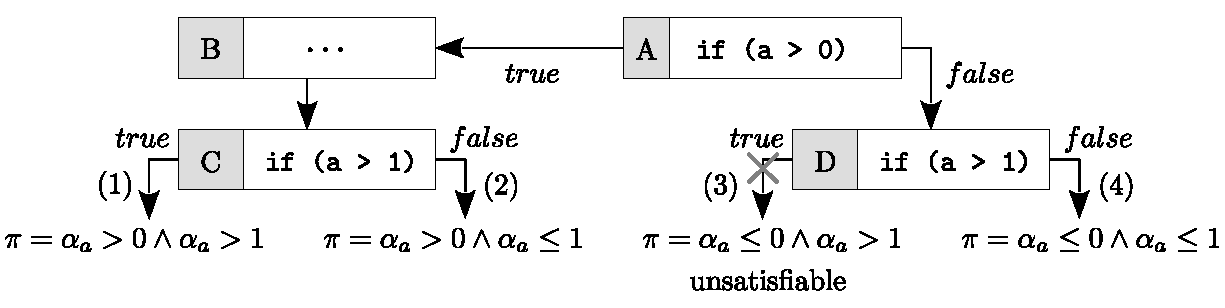
\includegraphics[width=1.0\columnwidth]{images/eager-evaluation} 
    %\label{fig:sub1}
    \vspace{-5mm}
    \caption{}
  \end{subfigure}%
  \vspace{-2mm}
  \caption{Pruning unrealizable paths example: (a) Code fragment; (b) symbolic execution of the code fragment: the {\em true} branch at node D is not explored since its path constraints $(\alpha_a \leq 0 \wedge \alpha_a > 1)$ are not satisfiable.}
  \label{fig:eager-evaluation}
\end{figure}

\myedit{A first natural technique} for reducing the path space is to invoke the constraint solver at each branch, pruning unrealizable branches: if the solver can prove that the logical formula given by the path constraints of a branch is not satisfiable, then no assignment of the program input values could drive a real execution towards that path, which can be safely discarded by the symbolic engine without affecting soundness. 

\boxedexample{Consider the example shown in Figure~\ref{fig:eager-evaluation} and assume that {\tt a} is a local variable bound to an unconstrained symbol $\alpha_a$. A symbolic engine would start the execution of the code fragment of Figure~\ref{fig:eager-evaluation}a by evaluating the branch condition $a > 0$. Before expanding both branches, the symbolic engine queries a constraint solver to verify that no contradiction arises when adding to the path constraints $\pi$ the {\em true} branch condition ($\alpha_a > 0$) or the {\em false} branch condition ($\alpha_a \leq 0$). Since both paths are feasible, the engine forks the execution states B and D (see Figure~\ref{fig:eager-evaluation}b). A similar scenario happens when the engine evaluates the branch condition $a > 1$. However, since $\alpha_a$ is not unconstrained anymore, some contradictions are actually possible. The engine queries the solver to check the following path constraints: (1) $\alpha_a > 0~\wedge~\alpha_a > 1$, (2)~$\alpha_a > 0~\wedge~\alpha_a \leq 1$, (3) $\alpha_a \leq 0~\wedge~\alpha_a > 1$, and (4) $\alpha_a \leq 0~\wedge~\alpha_a \leq 1$. The formula $\alpha_a \leq 0 \wedge \alpha_a > 1$, however, does not admit a valid solution and therefore the related path can be safely dropped by the engine. %On the other hand, other paths admit a valid solution and can be further explored by the engine.
}

\noindent This approach is commonly referred to as {\em eager evaluation} of path constraints, since constraints are eagerly checked at each branch, and is typically the default in most symbolic engines. We refer to Section~\ref{se:constraint-solving} for a discussion of the opposite strategy, called {\em lazy evaluation}, aimed at reducing the burden on the constraint solver.

% From warm-up example\mynote{IF: I removed from the warm up the non-forking case. Must be explained here}:

% The evaluation of a conditional branch ${\tt if}~e~{\tt then}~s_{true}~{\tt else}~s_{false}$ affects the path constraint. Two scenarios are possible:
%     \begin{enumerate}
%       \item {\em Non-forking}: if $e$ is evaluated as always true (resp., false) under the assumptions in the current state, the proper branch is taken and the symbolic execution advances to $s_{true}$ (resp., $s_{false}$);
%       \item {\em Forking}: if $e$ cannot be evaluated without instantiating values for one or more of its symbols, the symbolic execution is forked by creating two execution states with path constraints $pct_{true}$ and $pct_{false}$, respectively, corresponding to the two {\tt if} branches. Namely, $pct_{true}=pct \wedge e_s$ and $pct_{false}=pct \wedge \neg e_s$, where $e_s$ is a symbolic expression obtained by evaluating $e$. 
% %        \[ (s_{true}, pc_{true}) \text{ where } pc_{true} = pc \wedge e \]
% %        \[ (s_{false}, pc_{false}) \text{ where } pc_{false} = pc \wedge \neg e \]
%     Symbolic execution proceeds on both states in parallel.
%     \end{enumerate}

\subsection{Function calls} 
\label{ss:functions}

\mytempedit{Function calls and loops are the main sources of path explosion. Many works have attempted to capture similarities across distinct function invocations or loop iterations by devising {\em summarization} strategies that prevent repeated explorations of a code portion, or by inferring {\em invariants} that inductively describe properties of a computation. In this section we present a number of prominent techniques for handling function calls, treating loops separately in Section~\ref{ss:loops}.}

% allowing the symbolic executor
A function $f$ may be called multiple times during an execution, either at the same calling context or at different ones. Differently from traditional symbolic execution, which requires to symbolically execute $f$ at each invocation, the {\em compositional} approach described in~\cite{G-POPL07} dynamically generates {\em function summaries}, allowing \mynote{I: si intende function inputs?} the executor to effectively reuse prior discovered analysis results. \mytempedit{Proposed for concolic executors, the technique captures the effects of a function invocation with a formula $\phi_w$ that conjoins \mynote{I: Perche' w a pedice? Cosa indica?} constraints on the inputs, describing equivalence classes of concrete executions, with constraints observed on the output. A function summary is a propositional logic formula defined as the disjunction of $\phi_w$ formulas from distinct classes, and feasible inter-procedural paths are  modeled by composing symbolic executions of intra-procedural ones.
%
Compositional symbolic execution has been extended in~\cite{AGT-TACAS08}: summaries are generated as first-order logic formulas with uninterpreted functions, allowing the formation of incomplete summaries (i.e., capturing only a subset of the paths within a function) that can be expanded on demand during the inter-procedural analysis as more statements get covered. 
%
\mytempedit{
\cite{CFS-PLDI09} makes a step further by describing an algorithm for generalizing symbolic summaries, effectively enhancing their reuse in practice.
}

%A similar idea has been also proposed in~\cite{BCE-TACAS08}. The main intuition is that,
\cite{BCE-TACAS08} explores a different flavor of summarization, exploiting the following intuition:
}
if two program states differ only for some program values that are not read later, the executions generated by the two states will produce the same side effects. Side effects of a code fragment can be therefore cached and possibly reused later.

% proved to be weak
% is a static checker based on verification conditions (i.e., logical formulas capturing correctness properties in a program) that
\mytempedit{
\myparagraph{Related Work}
Function summaries \mynote{Da rivedere con Daniele o Emilio} have largely been employed in static and dynamic program analysis techniques, especially in program verification. A number of such works offer interesting opportunities to advance the state of the art in symbolic execution. For instance, the Calysto static checker~\cite{CALYSTO-ICSE08} walks the call graph of a program to construct a symbolic representation of the effects of each function, i.e., return values, writes to global variables, and memory locations accessed depending on its arguments. Each function is processed once, possibly inlining effects of small ones at their call sites. Static checkers such as Calysto~\cite{CALYSTO-ICSE08} and Saturn~\cite{SATURN-POPL05} trade scalability for soundness in summary construction, as they unwind loops only to a small number of iterations: such techniques could then only be used for loop-free \mynote{perche' loop-free? Poche iterazioni non sono supportate?} functions in the symbolic execution setting. More fine-grained summaries are constructed in~\cite{RACERX-SOSP03} by taking into account different input conditions using a summary cache for memoizing the effects of a function.

\cite{SFS11} proposes a technique to extract function summaries for model checking where multiple specifications are typically checked one a time, so that summaries can be reused across verification runs. In particular, they are computed as over-approximations using interpolation -- a technique that we discuss in detail in Section~\ref{ss:interpolation} -- and refined across runs when too weak. The strength of this technique lies in the fact that an interpolant-based summary can capture all the possible execution traces through a function in a more compact way than the function itself. The technique has later been extended to deal with nested function calls in~\cite{SFS12}, which discusses an useful application in incremental update checking of programs. 
}

\subsection{Loops} 
\label{ss:loops}

Loops \mynote{I: sposterei queste 4 righe e l'esempio in 5.3: controindicazioni?} are one of the main causes of path explosion: each iteration of a loop can be seen as an {\tt if-goto} statement, leading to a conditional branch in the execution tree. If the loop condition involves one or more symbolic values, the number of generated branches may be potentially infinite. 

\begin{figure}[t]
\begin{center}
\begin{tabular}{c}
\begin{lstlisting}[basicstyle=\ttfamily\scriptsize]
1.  int x = sym_input(); // e.g., read from file
2.  while (x > 0) {
3.     x = sym_input();  
4.  }
\end{lstlisting}
\end{tabular}
\end{center}
\vspace{-2mm}
\caption{Loop example with input read from the environment~\protect\cite{CS-CACM13}.}
\label{fi:example-loop}
\end{figure}

\vspace{-2pt} % TODO
\boxedexample{Consider the code fragment of Figure~\ref{fi:example-loop}~\cite{CS-CACM13}, where \texttt{sym\_input()} is an external routine that interacts with the environment (e.g., by reading input data from a network) and returns a fresh symbolic input. The path constraint set at any final state has the form: 
\[ \pi = \left ( \bigwedge_{i \in [1, k]} \alpha_i > 0 \right ) \wedge (\alpha_{k+1} \leq 0) \] 
where $k$ is the number of iterations and $\alpha_i$ is the symbol produced by \texttt{sym\_input()} at the $i$-th iteration.}



The problem of path explosion due to symbolic execution of loops has been attacked from different sides. \mytempedit{In this section we review the main approaches in the literature, and explore connections with other program analysis and verification techniques.}

\mytempedit{\myparagraph{Bounded Exploration}}
A first natural strategy adopted by many symbolic engines is to limit the loop exploration up to a certain number of iterations. Obviously, this may lead to missing interesting paths in the program. For this reason, some works (e.g., {\sc AEG}~\cite{AEG-NDSS11}) have also considered the opposite strategy, allowing the engine to fully explore some loops. To mitigate the path explosion problem, only a single instance of the symbolic executor is allowed to fully unroll a loop, while other instances conservatively explore other paths. This approach has been shown to be effective in some application contexts such as security (e.g., identification of buffer overflows) where interesting behavior may be observed at the loop boundaries.

By using static or dynamic analysis techniques, it may be possible to derive properties over a loop that can be exploited by the symbolic engine to significantly prune branching paths. For instance, knowledge of the exact number of loop iterations - or at least a constant upper bound on it - can significantly help the engine. Section~\ref{precontioned-symbolic-execution} provides a more general discussion of how preconditions can help symbolic execution.

\mytempedit{\myparagraph{Summaries}}
\cite{GL-ISSTA11} presents a technique that automatically derives partial summarizations for loops. A loop summarization is similar to a function summary, using a set of preconditions and a set of postconditions. These are computed dynamically during the symbolic execution by reasoning on the dependencies among loop conditions and symbolic variables. As soon as a loop summary is computed, it is cached for possibly subsequent reuse. This not only allows the symbolic engine to avoid redundant executions of the same loop under the same program state, but also makes it possible to generalize the loop summary to cover even different executions of the same loop that run under different conditions. A main limitation of this approach is that it can generate summaries only for loops that iteratively update symbolic variables across loop iterations by adding a constant, non-zero amount.

\mytempedit{
  % still WIP
 \myedit{Another} crucial limitation of \myedit{early summarization} works is that in general they cannot handle nested loops as well as {\em multi-path loops}, i.e., loops that contain one or more branches. In the last few years, the latter scenario has been effectively tackled first by S-Looper~\cite{XX-ISSTA15} and later by Proteus~\cite{XX-FSE16}. S-Looper targets loops that traverse a string, without modifying it, and that have branch conditions related to the traversed string or other loop induction variables. Proteus has made a step further by proposing a more general framework for summarization of multi-path loops. First, it classifies loops based on the patterns of value changes, i.e., whether the loop variables are induction or non-induction, and based on the patterns of path interleaving, i.e., whether the path interleaving can be considered {\em sequential}, {\em periodic}, or {\em irregular}. In order to perform loop classification, Proteus constructs a flowgraph of the sliced loop program. Loop slicing is performed exploiting the program dependence graph (PDG), which combines the control flow graph (CGF) and the data dependencies of the loop. The flowgraph is then analyzed and the loop classified. Depending of the type of the loop, different strategies are used for generating a disjunctive loop summarization (DLS). Intuitively, a DLS is the union of all the trace summaries for a loop. For instance, loops that contain only induction variables and that have a path interleaving with a periodic pattern are summarized by first constructing the path dependency automaton (PDA) of the loop, then by summarizing the effect of distinct paths (periods) of the cycle and finally by relating these effects to the execution number of the loop. Although not all types of loops can be summarized by Proteus, it still can produce approximated loop summaries for many different types, which could be useful in practice. Precise summarization of multi-path loops with non-induction variables or with an irregular pattern, or even worse summarization of nested loops, still remain an open research problem. 
}

\mytempedit{\myparagraph{Invariants}
Loop invariants play a key role in verifiers that can prove programs correct against their full functional specification. An invariant is not just a quantity that remains unchanged throughout executions of the loop body, but an inductive property that holds when the loop is first entered and is preserved for an arbitrary number of iterations~\cite{FMV-CSUR14,GFM-TSE15}. Leveraging invariants can be beneficial to symbolic executors, in order to compactly capture the effects of a loop and reason about them. Unfortunately, we are not aware of symbolic executors taking advantage of this approach. One of the reasons might lie in the difficulty of computing loop invariants without requiring manual intervention from domain experts. In fact, lessons from the verification practice suggest that providing loop invariants is much harder compared to other specification elements such as method pre/post-conditions.

% a number of works [...] and might be
However, many researchers have recently explored techniques for inferring loop invariants automatically or with little human help~\cite{FMV-CSUR14}, which might be of interest for the symbolic execution community.
%
% that rank all -> over all
{\em Termination analysis} has been applied to verify program termination for industrial code: a formal argument is typically built by using one or more ranking functions over all the possible states in the program such that for every state transition, at least one function decreases~\cite{CPR-PLDI06}. Ranking functions can be constructed in a number of ways, e.g., by lazily building an invariant using counterexamples from traversed loop paths~\cite{GMR-PLDI15}. Another way to construct a termination argument is to reason over loop-free code by using loop summaries based on transition invariants~\cite{TSW-TACAS11}. It has been observed that most loops in practice have relatively simple termination arguments~\cite{TSW-TACAS11}, and discovered invariants may thus be too simple for a verification setting~\cite{GFM-TSE15}. However, a constant or parametric bound on the number of iterations may be computed from a ranking function and an invariant~\cite{GMR-PLDI15}.
%
{\em Predicate abstraction} is as a form of abstract interpretation over a domain constructed using a given set of predicates, and has been used to infer universally quantified loop invariants~\cite{FQ-POPL02}, which are useful when manipulating arrays. Predicates can be heuristically collected from the code or supplied by the user; it would be interesting to explore whether an executor might provide useful predicates from a symbolic exploration of the code. {\em LoopFrog}~\cite{LOOPFROG-ATVA08} replaces loops using a symbolic abstract transformer with respect to a set of abstract domains, obtaining a conservative abstraction of the original code. Abstract transformers are computed starting from the innermost loop, and the output is a loop-free summary of the program that can be handed to a model checker for verification. This approach can also be applied to non-recursive function calls, and might deserve further investigation in symbolic executors. Loop invariants can also be extracted using {\em interpolation}, a general technique that has already been applied in symbolic execution for different goals as we discuss in the next section. More generally, we believe that modern advances in invariant generation can provide potential solutions for handling loops more efficiently in a symbolic executor.
}

On the other hand, symbolic execution has proven useful to derive loop invariants. For instance, if a program contains an assertion after the loop, the approach presented in~\cite{PV-SPIN04} works backwards from the property to be checked and it iteratively applies approximation to derive loop invariants. The main idea is to pick the asserted property as the initial invariant candidate and then to exploit symbolic execution to check whether this property is inductive. If the invariant cannot be verified for some loop paths, it is replaced by a different invariant. The next candidate for the invariant is generated by exploiting the path constraints for the paths on which the verification has failed. Additional refinements steps are performed to guarantee termination. % [D] say weakness in not being able to find invariants that do not directly depends on the path conditions?

%Nevertheless, even symbolic execution can be used to derive loop invariants. Indeed, if a program contains an assertion after the loop, the approach presented in~\cite{PV-SPIN04} works backwards from the property to be checked and it iteratively applies approximation to derive loop invariants. The main idea is to pick the asserted property as the initial invariant candidate and then to exploit symbolic execution to check whether this property is inductive. If the invariant cannot be verified for some loop paths, it is replaced by a different invariant. The next candidate for the invariant is generated by exploiting the path constraints for the paths on which the verification has failed. Additional refinements steps are performed to guarantee termination.
%this can be exploited by a symbolic engine for automatically discovering some invariants over the loop. In~\cite{PV-SPIN04}, this is achieved by iteratively using \mynote{[D] Define?} invariant strengthening and approximation techniques. 

\mytempedit{\myparagraph{Other Techniques}}
% technique of a different flavor
\cite{SST-ATVA13} introduces a \myedit{different flavor of symbolic execution} that analyzes cyclic paths in the control flow graph of a given program and produces {\em templates} that declaratively describe the program states generated by these portions of code \myedit{as} a \myedit{\em compact} symbolic execution tree. By exploiting templates, the symbolic execution engine needs to explore a significantly reduced number of program states. A drawback of this approach is that templates introduce quantifiers in the path constraints: in turn, this may significantly increase the burden on the constraint solver.

% [D] I don't think mentioning trip counts adds value to the discussion, better keep thing simple
% By relating {\em trip counts} (i.e., number of iterations for loops) with features of the program input
It has also been observed that loop executions may strictly depend on input features. {\em Loop-extended symbolic execution}~\cite{SPM-ISSTA09} is able to effectively explore a loop whenever a grammar describing the input program is available. Relating the number of iterations with features of the program input can guide the exploration of the program states generated by a loop.


% ---------------------------------------------------------------------------------------------------
\subsection{Symbolic Execution with Interpolation} 
\label{ss:interpolation}
\mytempedit{
Modern SAT solvers rely on a mutual reinforcing combination of search and deduction, using the latter to drive the former away from a conflict when it becomes blocked. In a similar manner, symbolic execution can benefit from {\em interpolation} techniques to derive properties from program paths that did not show a desired property, so to prevent the execution from exploring other paths that would lead to a failure in the same way.

{\em Craig interpolants}~\cite{Craig1957} allow deciding what information about a formula is relevant to a property. Assuming a formula $P\rightarrow Q$ holds in some logic, it is possible to construct an interpolant $I$ such that $P\rightarrow I$ and $I\rightarrow Q$ are valid, and every non-logical symbol in $I$ occurs in both $P$ and $Q$. In program verification, interpolants are typically devised as follows: given a refutation proof for an unsatisfiable formula $P\wedge Q$, an interpolant $I$ can be constructed such that $P\rightarrow I$ is valid and $I\wedge Q$ is unsatisfiable.

Interpolation has largely been employed in model checking, predicate abstraction, predicate refinement, theorem proving, and other areas. For instance, interpolants provide a methodology to extend {\em bounded model checking} -- which aims at the falsification of safety properties of a program for which the transition relation is unrolled up to a given bound -- to the unbounded case. In particular, since bounded proofs often contains the ingredients of unbounded proofs, interpolation can help construct an over-approximation of all reachable final states from the refutation proof for the bounded case, obtaining an over-approximation that is strong enough to prove absence of errors.
% given a refutation proof for the bounded case, 
% that is strong enough to provide guarantees on the absence of errors, but also loose enough to allow for an efficient computation.

\myparagraph{Path Subsumption}
Symbolic execution with interpolation has been proposed for software verification as an alternative to model checking-based techniques. Given a program annotated with assertions for bug conditions, interpolation can be used to tackle the path explosion program by annotating program locations with conditions summarizing previously explored paths, so that every time a branch is encountered, the executor can check whether it is subsumed by a previous exploration. In a best-case scenario, this approach can reduce the number of visited paths exponentially. 

\cite{McMillan10} proposes an algorithm to annotate branches and program locations with labels such that if they are implied by the current state, no error location can be reached from there. Interpolation is used to construct weak labels that allow for an efficient computation of implication. \cite{YYG15} proposes a similar redundancy removal method called {\em postconditioned symbolic execution}, where  program locations are annotated with a postcondition, i.e., the {\em weakest precondition} summarizing path suffixes from previous explorations. The intuition here is that the weaker the interpolant it, the more likely it would enable path subsumption. Postconditions are constructed incrementally from fully explored paths and propagated backwards. When a branch is encountered, the corresponding postcondition is negated and added to the path constraints, which become unsatisfiable if the path is subsumed by previous explorations.

The soundness of path subsumption relies on the fact that an interpolant computed for a location captures the entirety of paths going through it. Thus, the path selection strategy plays a key role in enabling interpolant construction: for instance, DFS is very convenient as it allows exploring paths in full quickly, so that interpolants can be constructed and eventually propagated backwards; BFS instead hinders subsumption as interpolants may not available when checking for redundancy at branches as similar paths have not been explored in full yet. \cite{JMN13} proposes a novel strategy called {\em greedy confirmation} that decouples the path selection problem from the interpolant formation, allowing users to benefit from path subsumption when using heuristics other than DFS. Greedy confirmation distinguishes betweens nodes whose trees of paths have been explored in full or partially: for the latter, it performs limited traversal of additional paths to enable interpolant formation.

Interpolation has been proven to be useful for allowing to explore larger portions of a complex program within a given time budget. Typically, the overhead of interpolation - which can be performed within the SMT solver or using a dedicated engine - slows down the exploration in the early stages, then its benefits eventually start to pay off, allowing for a much faster exploration~\cite{JMN13}. \cite{YYG15} claims that such path redundancy is abundant and widespread in real-world applications.

\myparagraph{Subsumption with Unbounded Loops}
The remaining challenge is due to unbounded loops, which make it harder to perform sound subsumption at program locations in it due to the very large number of paths that can go through them. \cite{McMillan10} devises an iterative deepening strategy that unwinds loops until a fixed depth and tries to compute interpolants that are {\em loop invariant}, so that they can be used to prove the unreachability of error nodes in the unbounded case. This method however may not terminate for programs that require disjunctive loop invariants. \cite{JNS11} thus proposes a strategy to compute speculative invariants strong enough to make the symbolic execution of the loop converge quickly, but also loose enough to allow for path subsumption whenever possible. In a follow-up work~\cite{JMN12}, loop invariants are discovered separately during the symbolic execution using a widening operator, and weakest preconditions for path subsumption are constructed such that they are entailed by the loop invariants.

We believe that the idea of using abstract interpretation in this setting -- originally suggested in~\cite{JSV09} -- deserves further investigation, as it can benefit from its many applications in other program verification techniques, and is amenable to an efficient implementation in mainstream symbolic executors, provided that the constructed invariants are accurate enough to capture the (un)rechability of error nodes.




%control-flow branches and program locations with labels, representing a condition under which no error locations can be reached. Labels are initially empty and constructed in a bottom-up fashion: once a path leading to an error has proven to be unfeasible,
%interpolation is used to compute a weaker formula that becomes the annotation for the last taken branch. As branches are explored,  
%has been fully explored and no error is found, interpolation is used to compute a weaker formula that 
%interpolation is used to compute conditions that are eventually propagated to their ancestors. 

}
% ---------------------------------------------------------------------------------------------------
\subsection{Under-Constrained Symbolic Execution} 
\label{under-constrained}

A possible approach to avoid path explosion is to cut the code to check, say a function, out of its enclosing system and check it in isolation. Lazy initialization with user-specified preconditions (Section~\ref{ss:complex-objects}) follows this principle in order to automatically reconstruct complex  data structures. However, taking a code region out of an application has proven to be quite difficult due to the entanglements with the surrounding environment~\cite{ED-ISSTA07}.

% certain values (e.g., a null pointer)
The main issue is that errors detected in a function analyzed in isolation may be false positives, as the input may never assume certain values when the function is executed in the context of a full program. Some prior works, e.g., {\sc Check 'n' Crash}~\cite{CS-ICSE05}, first analyze the code in isolation and then test the generated crashing inputs using concrete executions.

%{\em Under-constrained symbolic execution}~\cite{ED-ISSTA07} is a twist on symbolic execution that allows for the analysis of a function in isolation by marking some symbolic inputs as {\em under-constrained}. Intuitively, a symbolic variable is under-constrained when in the analysis we do not account for constraints on its value that should have been collected along the path prefix from the program's entry point to the function to analyze. Under-constrained variables have the same semantics as classic symbolic variables except when used in an expression that can cause an error to occur. In particular, an error is reported only if all the solutions for the currently known constraints on the variable cause it to occur, i.e., the error is context-insensitive and thus a true positive. Otherwise, its negation is added to the path constraints and execution resumes as normal. This choice can be regarded as an attempt to reconstruct preconditions from the checks inserted in the code: any subsequent action violating an added negated constraint will be reported as an error.

\mytempedit{
{\em Under-constrained symbolic execution}~\cite{ED-ISSTA07} is a twist on symbolic execution that allows for the analysis of a function in isolation by marking its symbolic inputs, as well as any global data that may affect its execution, as {\em under-constrained}. In practice, a symbolic engine can automatically mark data as under-constrained without manual intervention by tracing memory accesses and by identifying their location (e.g., a function input can be detected when a read memory access is perfomed on some uninitialized data located into the stack). Intuitively, a symbolic variable is under-constrained when in the analysis we do not account for constraints on its value that should have been collected along the path prefix from the program's entry point to the function to analyze. Under-constrained variables have the same semantics as classic fully-constrained symbolic variables except when used in an expression that can cause an error to occur. In particular, an error is reported only if all the solutions for the currently known constraints on the variable cause it to occur, i.e., the error is context-insensitive and thus a true positive. Otherwise, its negation is added to the path constraints and execution resumes as normal. This choice can be regarded as an attempt to reconstruct preconditions from the checks inserted in the code: any subsequent action violating an added negated constraint will be reported as an error. In order to keep this analysis correct, marks must be propagated between variables whenever any expression involves both under-constrained and fully-constrained values. For instance, any comparison such as {\tt a > b}, where {\tt a} is under-constrained while {\tt b} is fully-constrained, forces the engine to propagate the mark from {\tt a} to {\tt b}, similarly as done by a taint-analysis engine when handling tainted values. Marks are typically tracked by an engine using a shadow memory.
}

%{\em Under-constrained symbolic execution}~\cite{ED-ISSTA07} is a twist on symbolic execution that allows for the analysis of a function in isolation by marking symbolic inputs for which preconditions are missing as {\em under-constrained}. Intuitively, missing preconditions are the constraints on the variable yielded along the path prefix from the program's entry point to the function. Under-constrained variables have the same semantics as classic symbolic variables except when used in an expression that can cause an error to occur. In this case, an error is reported only if all the solutions for the currently known constraints on the variable cause it to occur, i.e., the error is context-insensitive and a true positive. Otherwise, its negation is added to the path constraints and execution resumes as normal. This choice can be regarded as an attempt to reconstruct preconditions from the checks inserted in the code. Any subsequent action violating an added negated constraint will be reported as an error.

Although this technique is not sound as it may miss errors, it can still scale to find interesting bugs in larger programs. Also, the application of under-constrained symbolic execution is not limited to functions only: for instance, if a code region (e.g., a loop) may be troublesome for the symbolic executor, it can be skipped by marking the locations affected by it as under-constrained. \mytempedit{Since in general it's not easy to understand which data could be affected by the execution of some skipped code, manual annotation may be needed in order to keep the analysis correct.}

% ---------------------------------------------------------------------------------------------------
\subsection{Preconditioned Symbolic Execution}%\mynote{[D] Entirely rewritten}
\label{precontioned-symbolic-execution}

% input state space
{\sc AEG}~\cite{AEG-NDSS11} proposes {\em preconditioned symbolic execution}, a technique for reducing the number of explored states by directing the exploration to a subset of the input space that satisfies a precondition predicate. The rationale is to focus on inputs that may lead to certain behaviors of the program.
For instance, we may be interested in narrowing down the exploration to inputs of maximum size to reveal potential buffer overflows. Preconditioned symbolic execution trades soundness for performance: well-designed preconditions should not be too specific, as they may miss interesting paths, and not too generic, since the speedups resulting from the space state reduction may not be significant enough to be of practical interest. Instead of starting from an empty path constraints set, the approach adds the preconditions to the initial $\pi$ so that the rest of the exploration will skip branches that do not satisfy them. While adding more constraints to $\pi$ at initialization time is likely to increase the burden on the solver, which is required to perform a larger number of checks at each branch instruction, this may be largely outweighted by the performance gains due to the smaller state space to be explored.

\begin{figure}[t]
\centering
\begin{subfigure}[t]{.4\textwidth}
\begin{tabular}{c}
\begin{lstlisting}[basicstyle=\ttfamily\scriptsize]
// N symbolic branches 
if (input[0] < 42) [...]
[...]
if (input[N-1] < 42) [...]

// symbolic loop
strcpy(dest, input); 

// M symbolic branches
if (input[N] < 42) [...]
[...]
if (input[N+M-1] < 42) [...]
\end{lstlisting}
\end{tabular}
\caption{\label{fig:preconditioned}}
\end{subfigure}
\begin{subfigure}[t]{.4\textwidth}
\begin{tabular}{c}
\lstset{
   showlines=true
}
\begin{lstlisting}[basicstyle=\ttfamily\scriptsize]
1.  void foo(int x, int y) {
2.     if (x < 5)
3.        y = y * 2;
4.     else
5.        y = y * 3;
6.     return y;
7.  }

\end{lstlisting}
\end{tabular}
\caption{\label{fi:example-state-merging} }
\end{subfigure}
\caption{\label{fig:preconditioned-and-merge} (a) Preconditioned symbolic execution example~\protect\cite{AEG-NDSS11}; (b) State merging example}
\end{figure}

\noindent Typical preconditions considered in symbolic execution include:
\begin{itemize}
\item {\em Known length}: symbolic inputs are of known maximum length, e.g., a network packet has a fixed size, or static analysis can determine the input length;
%Static analysis techniques can be used to automatically determine this precondition.
\item {\em Known prefix}: symbolic inputs have a known prefix, e.g., a fixed header string such as the initial {\em magic code} in a binary, or a network packet header.
\item {\em Fully known}: all input bytes are concrete, leading to a concolic execution; it can be used, for instance, to generate a working exploit from a known crashing input. 
\end{itemize}

\boxedexample{Consider the code fragment in Figure~\ref{fig:preconditioned} where {\tt input} is an array of $s\ge n+m$ bytes. Without any precodition, the input space size is $256^s$, and up to $2^n\cdot s\cdot 2^m$ execution engine instances are needed, due to $n+m$ symbolic branches and up to $s$ loop iterations. The impact of preconditions on the state space size is as follows:
\begin{itemize}
  \item {\em Known length}: if we assume a string length $s$, i.e., the first $(s-1)$ bytes of {\tt input} are not $\setminus0$, the loop is concretized, and the state space size is reduced to $2^{n+m}$;
  \item {\em Known prefix}: if a prefix of $p<n$ bytes is known for {\tt input}, the first $p$ branches and $p$ loop iterations are concrete, and the state space size becomes $2^{n-p}\cdot s\cdot 2^m$;
  \item {\em Fully known}: as all input bytes are concrete, the state space size is trivially $1$.
\end{itemize}}

% [D] shall we mention that for prefixes also inequalities can be used, and that prefixes while they reduce the space size, they can lead to missing interesting states, e.g., malformed headers? I think it would be a bit too much detailed


% ---------------------------------------------------------------------------------------------------

%\subsection{Dynamic symbolic execution}
%Dynamic symbolic execution refers to a body of techniques that exploit execution with concrete values to explore [...].

% ---------------------------------------------------------------------------------------------------
\subsection{State Merging}

Several static program analysis techniques such as abstract interpretation merge states corresponding to different paths into a state that over-approximates them. In a precise symbolic execution, however, merging is not allowed to introduce any approximation or abstraction, and therefore can only change formulas to have them characterize sets of execution paths. In other words, a merged state will be described by a formula that represents the disjunction of the formulas that would have described the individual states if they were kept separate.

\boxedexample{Consider the function of Figure~\ref{fi:example-state-merging} and its symbolic execution tree shown in Figure~\ref{fig:example-state-merging}a. Initially (execution state $A$) the path constraints are {\em true} and input arguments {\tt x} and {\tt y} are associated with symbolic values $\alpha_x$ and $\alpha_y$, respectively. Line~2 contains a conditional branch and the execution is forked: depending on the branch taken, a different statement is evaluated next and different assumptions are made on symbol $\alpha_x$ (execution states $C$ and $D$, respectively). After expanding every execution state until the {\tt return} at line 6 is reached on all branches, the symbolic execution tree gets populated with two additional states $D$ and $E$. If a symbolic execution engine desires to reduce the number of active states, then state merging can be performed. For instance, Figure~\ref{fig:example-state-merging}b shows the symbolic execution DAG for the same piece of code when a state merging operation is performed before evaluating the {\tt return} statement at line 6: $D'$ is now a merged state that fully captures the former execution states $D$ and $E$ using the $ite$ expression $ite(\alpha_x<5, 2*\alpha_y, 3*\alpha_y)$ (Section~\ref{ss:fully-symbolic-memory}). 
%Indeed, the $ite(\texttt{c}, \texttt{t}, \texttt{f})$ expression introduced in the symbolic store $\sigma$ is a short term for an {\tt if-then-else} expression and means that if the condition {\tt c} is verified then {\tt t} holds, otherwise {\tt f} must be assumed as true. Nonetheless, $ite$ expressions are often just syntactic sugar for disjunctive formulas and are commonly supported by most prominent constraint solvers. For instance, in the context of propositional logic the $ite(\texttt{c}, \texttt{t}, \texttt{f})$  expression could be replaced with the formula $(\texttt{c} \wedge \texttt{t}) \vee (\neg\texttt{c} \wedge \texttt{f})$ . However, since the symbolic store in our model should return an integer value for variable $y$ rather than a boolean value, following the idea presented in~\cite{KP-PP05}, the $ite$ expression could be translated into the expression $((\alpha_x < 5) * (2 * \alpha_y)) + (\neg(\alpha_x < 5) * (3 * \alpha_y))$ that evaluates\footnote{We are assuming that the result of a comparison maps to integer values 0 or 1.} to the actual value of {\tt y} based on the branch condition at line 2. 
%Indeed, the condition $(\alpha_x < 5)$ could be either true or false, yielding to only one of two possible values of $y$. 
Note that the path constraints of the execution states $D$ and $E$ can be merged into the disjunction formula $\alpha_x < 5 \vee \alpha_x \geq 5$ and then simplified to $true$ in $D'$.
}

%$(\alpha_x < 5 \wedge 2 * \alpha_y) \vee (\neg(\alpha_x < 5) \wedge 3 * \alpha_y)$



% Constructing Efficient Formal Models from High-Level Descriptions Using Symbolic Simulation

%As depicted by the symbolic execution tree shown in Figure~\ref{fig:example-state-merging}, when {\tt foo} is symbolically executed, the two input parameters {\tt x} and {\tt y} are mapped to the symbols  Whenever the branch condition on line 2 is evaluated, the two parallel execution states B and C are generated. Accordingly to taken branch, a different line of code is then evaluated, leading to execution states D and E. 


%In the branch where $\alpha_a\neq 0$, variable {\tt y} is assigned with ${\tt x}+3$, obtaining $y\mapsto 4$ in state $E$ because $x\mapsto 1$ in state $C$. In general, arithmetic expression evaluation simply manipulates the symbolic values.

%\noindent A symbolic execution engine may perform state merging in the following way:\noindent where {\em ite} represents an {\tt if-then-else} statement and $\bot$ a non-taken branch.

\begin{figure}[t]
  \vspace{-3mm}
  \centering
  \begin{subfigure}{.5\textwidth}
    \centering
    \hspace{-5mm}
    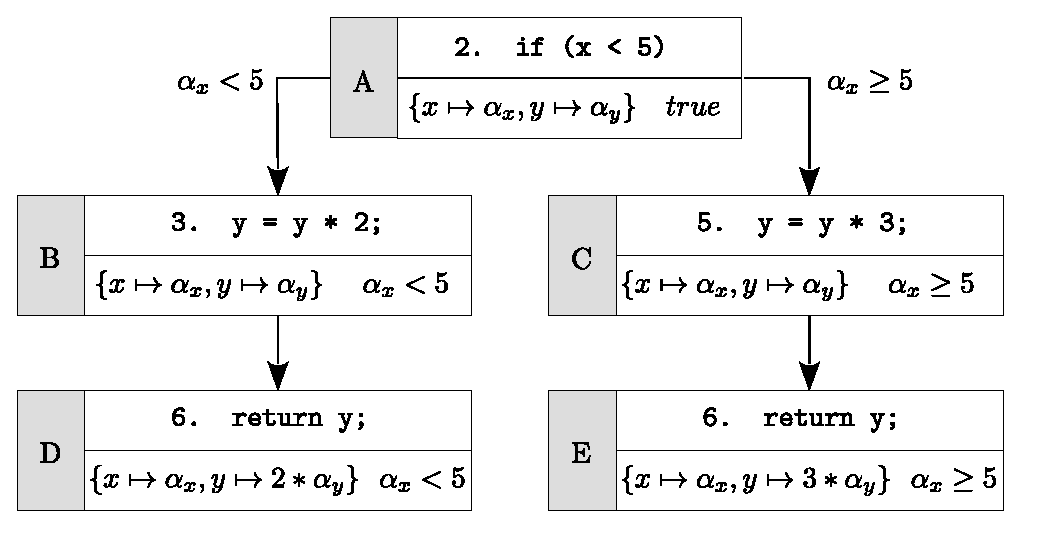
\includegraphics[width=1.05\columnwidth]{images/state-merging} 
    %\label{fig:sub1}
    \vspace{-6.5mm}
    \caption{}
  \end{subfigure}%
  \begin{subfigure}{.5\textwidth}
    \centering
    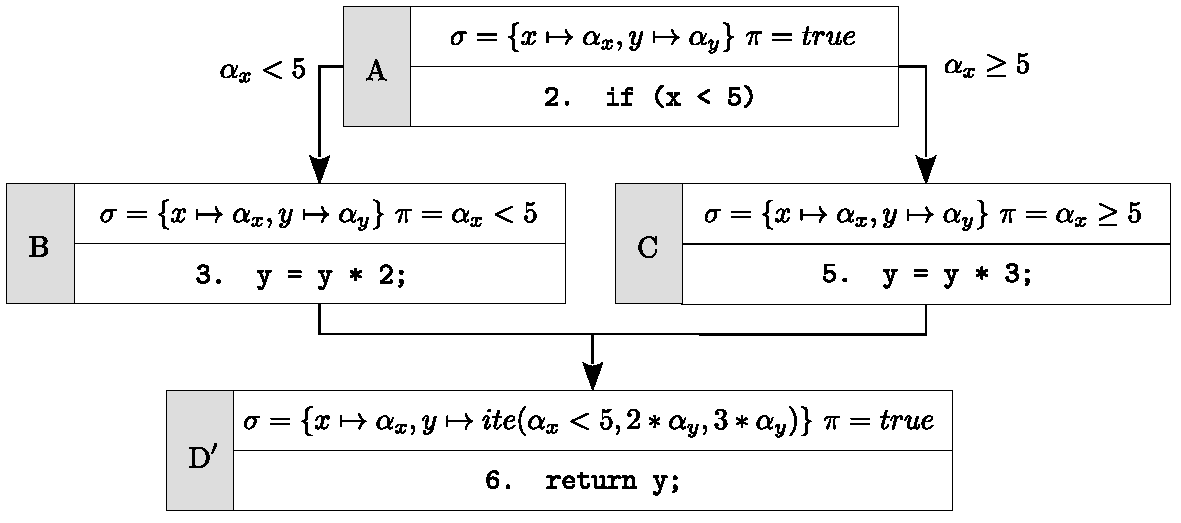
\includegraphics[width=1.05\columnwidth]{images/state-merging-2} 
    %\label{fig:sub2}
    \vspace{-4mm}
    \caption{}
  \end{subfigure}
  \vspace{-3mm}
  \caption{Symbolic execution of function \texttt{foo} of Figure~\ref{fi:example-state-merging}: (a) without state merging; (b) with state merging.}
  \label{fig:example-state-merging}
\end{figure}

%\vspace{-4pt} % TODO
\myparagraphnoperiod{Trade-Offs: to Merge or Not to Merge?} \mytempedit{In general, it makes sense to apply state merging whenever two symbolic states, that will next evaluate the same statement, are very similar in terms of their symbolic stores (i.e., they differ only for few elements). Given two states $(stmt_1,~\sigma_1,~\pi_1)$ and $(stmt_1,~\sigma_2,~\pi_2)$, the merged state can be constructed as $(stmt,~\sigma',~\pi_1 \vee \pi_2)$, where $stmt = stmt_1 = stmt_2$, $\sigma'$ is the merged symbolic store between $\sigma_1$ and $\sigma_2$ with {\em ite}-expressions that keep track of the differences between variables, and $\pi_1 \vee \pi_2$ which is the disjunction of the path constraints coming from the two merged states. Control-flow structures such as if-else statements (e.g., as the example discussed above) or simple loops often have successors which are very similar and thus represent very good candidates for state merging.}

Early works~\cite{G-POPL07,HSS-RV09} have shown that merging techniques effectively decrease the number of paths to explore, but also put a burden on constraints solvers, which typically encounter difficulties when dealing with disjunction. Merging can also introduce new symbolic expressions in the code, for instance when merging different concrete values from a conditional assignment into a symbolic expression over the condition. \cite{KKB-PLDI12} provides an excellent discussion of the design space of state merging techniques. At the one end of the spectrum, complete separation of the paths does not perform any merge and is used in search-based symbolic execution (Section~\ref{ss:heuristics}). At the other end, static state merging combines states at control-flow join points, thus essentially representing a whole program with a single formula. Static state merging is used in whole-program verification condition generators\iffullver{, e.g.,} ~\cite{SATURN-POPL05,CALYSTO-ICSE08}), \iffullver{which typically trade precision for scalability by, for instance, unrolling loops only once.}{which usually trade precision for scalability by, e.g., unrolling loops only once.}

%At the other end, static state merging combines states at control-flow join points after all subpaths leading to a join point have been explored.

%\mynote{Function summaries}

\myparagraph{Merging Heuristics} Intermediate merging solutions adopt heuristics to identify state merges that can speed the exploration process up. Indeed, generating larger symbolic expressions and possibly extra solvers invocations can outweigh the benefit of having fewer states, leading to poorer overall performance~\cite{HSS-RV09,KKB-PLDI12}. {\em Query count estimation}~\cite{KKB-PLDI12} relies on a simple static analysis to identify how often each variable is used in branch conditions past any given point in the CFG. The estimate is used as a proxy for the number of solver queries that a given variable is likely to be part of. Two states make a good candidate for merging when their differing variables are expected to appear infrequently in later queries. {\em Veritesting}~\cite{VERITESTING-ICSE14} implements a form of merging heuristic based on a distinction between easy and hard statements. Hard statements are those that involve indirect jumps, system calls, and other operations for which precise static analyses are difficult to achieve. Static merging is performed on sequences of easy statements, %which are represented as a single path 
whose effects are captured using $ite$ expressions, 
while per-path symbolic exploration is done whenever a hard-to-analyze statement is encountered. 

%identifies sequences of statements that do not contain system calls, indirect jumps, and other statements that are difficult to reason about statically, and represents them with a single formula as in static state merging. The approach is alternated with a per-path basis symbolic exploration every time a hard-to-analyze statement is encountered. 

\myparagraph{Dynamic State Merging} Ideally, in order to maximize the opportunities for merging, a symbolic execution engine should traverse a CFG so that a combined state for a program point can be computed from its predecessors, e.g., if the graph is acyclic, by following a topological ordering. However, this would prevent search exploration strategies aiming at prioritizing more ``interesting'' states over others. \cite{KKB-PLDI12} introduces {\em dynamic state merging} to identify opportunities for merging regardless of the exploration order imposed by the search strategy.
Suppose the symbolic engine maintains a worklist of states and a bounded history of their predecessors. When the engine has to pick the next state to explore, it first checks whether there are two states $s_1$ and $s_2$ from the worklist such that they do not match for merging, but $s_1$ and a predecessor of $s_2$ do. If the expected similarity between $s_2$ and a successor of $s_1$ is also high, the algorithm attempts a merge by advancing the execution of $s_1$ for a fixed number of steps. This captures the idea that if two states are similar, then also their respective successors are likely to become similar in a few steps. If the merge fails, the algorithm lets the search heuristic pick the next state to explore.

%This is useful, for instance, for unbounded loops for which search-based symbolic execution engines would employ search strategies that prioritize exploring new code over unrolling, while static state merging would require a depth-first exploration and thus fully unroll the possibly infinitely many iterations of the loop.

% ---------------------------------------------------------------------------------------------------
\subsection{Leveraging Program Analysis and Optimization Techniques}
\label{ss:program-analysis}

A deeper understanding of a program's behavior can help a symbolic engine to focus on promising states, e.g., by pruning uninteresting parts of the computation tree. Several classical program analysis techniques have been explored in the symbolic execution literature. Some prominent examples are listed below:

\begin{itemize}

\item {\em Program slicing} is a method that, starting from a subset of a program's behavior, extracts from the program the minimal sequence of instructions that faithfully represents that behavior~\cite{Weiser84}. This information can help a symbolic engine in several ways: for instance, given a program slice related to a target program point, symbolic exploration can be restricted to paths contained in the program slice. \iffullver{We discuss an example of use in Section~\ref{ss:auth-bypass}.}{}

\item {\em Taint analysis} attempts to check which variables of a program may hold values derived from potentially dangerous external sources such as user input. The analysis can be performed both statically and dynamically, with the latter yielding more accurate results. In the context of symbolic execution, taint analysis can help an engine skip execution paths that do not depend upon tainted values, effectively reducing the exploration state space~\cite{SAB-SP10}.

\item {\em Fuzzing} is a software testing technique that randomly mutates user-provided test inputs to cause crashes or assertion failures and find potential memory leaks. Fuzzing, as discussed in Section~\ref{ss:heuristics}, can be augmented with symbolic execution to collect constraints for an input and negate them to generate new inputs. On the other hand, a symbolic executor can be augmented with fuzzing to reach deeper states in the exploration more quickly and efficiently\iffullver{: we present two embodiments of this approach in Section~\ref{ss:bug-detection}.}{.\mynote{CD: consider citing fuzzers formerly in the apps section}}
  %\mynote{C: crossref: dynamic test generation}
  %\footnote{\cite{DRILLER-NDSS16} classifies offline symbolic executors such as {\sc DART} and {\sc SAGE} as {\em whitebox fuzzers}.}

\item {\em Branch predication} is a strategy for mitigating misprediction penalties in pipelined executions by avoiding jumps over very small sections of code: for instance, control-flow forking constructs such as the C ternary operator can be replaced with a predicated {\tt select} instruction. \cite{CCK-EUROSYS11} reports an exponential decrease in the number of paths to explore from the adoption of this strategy when cross-checking two implementations of a program using symbolic execution. % [D] alternative formulation: ~\cite{CCK-EUROSYS11} cross-checks two implementations of a program using symbolic execution and reports an exponential decrease in the number of paths to explore from the adoption of a simple form of this strategy; 
%  \item {\em source code analysis}: \mynote{TODO/drop?} extraction of input properties (e.g., size or contents of an array);

  \item {\em Type checking} can be effectively mixed with symbolic analysis~\cite{KCF-PLDI10};  for instance, type checking can determine the return type of a function that is difficult to analyze symbolically: such information can then potentially be used by the executor to prune certain paths\footnote{Interestingly,~\cite{KCF-PLDI10} discusses also how symbolic analysis can help a type checker. For instance, a symbolic engine can provide context-sensitive properties over a variable that would rule out certain type errors, improving the precision of the type checker.}.

  \item {\em State matching} determines whether an abstract state is subsumed by another, and can be used to analyze an under-approximation of a program's behavior. For instance, \cite{APV-SPIN06,VPP-ISSTA06} explore different heap shapes in the context of test generation for data structures, using subsumption checking to determine whether a symbolic state is being revisited. % ~\cite{XGM-ISSTA08} implements a different form of under-approximation: it looks for buffer overflows by having only a prefix of a buffer handled symbolically, and a symbolic length that may exceed the lenght of the prefix (any byte beyond the prefix is filled with concrete random data) - [D] I'm dropping this for now as we would have to call the item 'under-approximation' and change the first part of the text

\end{itemize}

\mytempedit{
\myparagraph{Classic Compiler Optimizations}
It has been also argued that program optimization techniques should be a first-class ingredient of practical implementations of symbolic execution, alongside widely accepted solutions such as search heuristics, state merging, and constraint solving optimizations~\cite{Cadar-FSE15}. In fact, program transformations can affect both the complexity of the constraints generated during path exploration and the exploration itself. For instance, precomputing the results of a function using a lookup table leads to a larger number of constraints in the path conditions due to memory accesses, while applying strength reduction for a multiplication by a constant results in a chain of addition operations that is more expensive for a constraint solver. Also, the way high-level {\tt switch} statements are compiled can significantly affect the performance of path exploration, while resorting to conditional instructions such as {\tt select} in LLVM or {\tt setcc} and {\tt cmov} in x86 can avoid expensive state forking by yielding {\em ite} expressions instead.

% D-THESIS14 superseded by DOZ-ISSRE15
%and none of them has tackled the analysis of binary programs.
While the effects of a compiler optimization can usually be predicted on the number or size of the instructions executed at run time, a similar reduction is not obvious in symbolic execution~\cite{DOZ-ISSRE15}, mostly because the constraint solver is typically used as a black-box. To the best of our knowledge, only a few works have attempted to analyze the impact of compiler optimizations on constraint generation and path exploration~\cite{WKC-HOTOS13,DOZ-ISSRE15}, leaving interesting open questions. \mynote{TODO: Move to 3.1?}Of a different flavor is the work presented in~\cite{PMZ-ISSTA17}, which explores transformations such as dynamic constant folding and optimized constraint encoding to speed up memory operations in symbolic executors based on theories of arrays (Section~\ref{ss:fully-symbolic-memory}).

\myparagraph{Further Directions}
We believe that the symbolic execution practice might also benefit from solutions that have been proposed for related problems in the program analysis realm. For instance, in the parallel computing community transformations such as {\em loop coalescing}~\cite{BGS-CSUR94} can restructure nested loops into a single loop by flattening the iteration space of their indexes. Such a transformation could potentially simplify a symbolic exploration, empowering search heuristics and state merging strategies. {\em Loop unfolding}~\cite{SK-SIGPLAN-NOTICES04} is another potentially interesting technique, as it allows exposing ``well-structured'' loops (e.g., showing invariant code, or having constants or affine functions as subscripts of array references) after peeling several iterations. {\em Program synthesis}~\cite{PR-POPL89} is a technique for automatic construction of a program satisfying a high-level specification, and in recent years has caught the attention of the verification community since it has been show how to find programs as a solution to SAT problems~\cite{Solar-Lezama08}. As we discussed in Section~\ref{se:environment-thirdparty}, \cite{JQF-ICSE16} has shown that program synthesis can be used to build models for complex Java components by abstracting away the details and entanglements of their implementations while capturing their functional behavior. In particular, the technique produces compact models by taking as inputs classes, methods and types from the framework, along with tutorial programs (typically those provided by the vendor) that exercise its parts. We believe this approach deserves further investigation in the context of the path explosion problem, as it could potentially be applied to software modules such as standard libraries to produce concise models that allow for a more scalable exploration of the search space. 
}

   %%%% DROPPED PARTS
    %\item {\em compositional techniques}: caching and reusing the analysis of lower-level function in subsequent computations. The main idea is to compute function summaries. See, e.g.,~\cite{G-POPL07,G-PLDI11,MS-TR07}.
   %%%% REWRITTEN PARTS
  %\item {\em phi-node folding} is a code transformation that can be used for statically merging some paths\mynote{E: relation with state merging?}. The main idea is to replace branches with predicated select instructions. Using this technique, the number of paths that must be explored by a symbolic engine can be significantly decreased. For instance,~\cite{CCK-EUROSYS11} used an aggressive variant of phi-node folding, called {\em if-conversion}~\cite{CCF-CGO03}, that allowed them to reduce the number of paths by an exponential factor on some benchmarks.
%\item \cite{DRILLER-NDSS16} is an example of {\em symbolic-assisted fuzzing}: their technique temporarily exploits concolic execution only when a fuzzer cannot generate a valid input to explore an uncovered branch.
 % \item {\em abstraction}~\cite{C-SEFM07} is a technique that may be used for computing {\em under-approximations} or {\em over-approximations} of a program state. This approach has been exploited in prior works~\cite{APV-SPIN06,VPP-ISSTA06,XGM-ISSTA08}\mynote{check these papers}. Since some of these works reason about state subsumption, they may be connected with the incremental solving optimization discussed in Section~\ref{constraint-optimizations}.
   %\item {\em type-checking}: \cite{KCF-PLDI10} shows how symbolic analysis can be effectively mixed with type-checking analysis. For instance, type-checking analysis can help a symbolic execution engine by detecting the type of an object (e.g., the type of a value returned by a {\em hard to reason} function). Although no assumption can be made on the value of the returned type, this information may still be useful for the symbolic engine (e.g., if the type has a fixed size, some preconditions can be set, possibly pruning some paths). Similarly, symbolic analysis can help a type checker. For instance, the symbolic engine may provide context-sensitive properties over a variable that clearly rules out type errors, reducing the number of false positive given by a traditional context-insensitive type checker.


\subsection{TODO}

\begin{itemize}[itemsep=2mm]

  \item {\em Constraint solver}: what can a constraint solver do in practice?
  %{\em What is a constraint solver in practice}? \\
 Constraint solvers suffer from a number of limitations. They can typically handle complex constraints in a reasonable amount of time only if they are made of polynomial expressions over their constituents. Symbolic execution engines normally implement a number of optimizations to make queries as much {\em solver-friendly} as possible, for instance by splitting queries into independent components to be processed separately or by performing algebraic simplifications.

  \item {\em Binary code}: what issues can arise when symbolically executing binary code?
  %what are the disadvantages of symbolically executing binary code?
 While the warm-up example of Section~\ref{symbolic-execution-example} is written in C, in several scenarios binary code is the only available representation of a program. However, having the source code of an application can make symbolic execution significantly easier, as it can exploit high-level properties (e.g., object shapes) that can be inferred statically by analyzing the source code.
  %(e.g., the maximum size of a buffer or the number of iterations for a loop).
   
\end{itemize}
%Depending on the specific application context of symbolic execution

\noindent Depending on the specific context in which symbolic execution is used, different choices and assumptions are made to address the questions highlighted above. Although these choices typically affect soundness or completeness, in several scenarios a partial exploration of the space of possible execution states may be sufficient to achieve the goal (e.g., identifying a crashing input for an application) within a limited time budget.

%different choices and assumptions are made to address the above questions. Although soundness and completeness of symbolic execution may be negatively affected by these choices, there are several application scenarios where a partial exploration of the possible execution states is sufficient for reaching the ultimate goal (e.g., identify a single input that crashes an application).
